 % The main file for CAMP reports
 % Don't put any content in here. 
 % Don't even include content files by using \input or \inlcude. 
 % Put your content to TEXT.TEX or include it there using \input.
 % Uses:
 %		SETTINGS.TEX		contains the settings for this document
 %		COMMANDS.TEX		contains commands which can be used while writing
 %		INFO.TEX			contains the author, title and so on for the cover
 %		COVER.TEX			formats the front cover of the document
 %		ABSTRACT.TEX		contains the abstract to be included (if needed)
 %		TEXT.TEX			contains the actual content of the document
 %		BIB.BIB				containt the BibTeX entries for the document
 


%% Draft document mode (with todos, no pictures just bounding box)
%\documentclass[draft,11pt,a4paper,bibtotoc,idxtotoc,headsepline,footsepline,footexclude,DIV13,oneside]{scrbook}
%% Final document mode (no todos, with pictures)
%\documentclass[final,11pt,a4paper,bibtotoc,idxtotoc,headsepline,footsepline,footexclude,DIV13,oneside]{scrbook}
%% Intermediate document mode (todos and pictures)
\documentclass[11pt,a4paper,bibtotoc,idxtotoc,headsepline,footsepline,footexclude,DIV13,oneside]{scrbook}

%\usepackage{epstopdf}
% KOMA-Optionen:
%  bibtotoc: include bibliography in table of contents
%  idxtotoc: include index in table of contents
%  headsepline: use horizontalline under heading
%  BCOR: binding correcion (Bindungskorrektur) (e.g.: BCOR5mm)
%  DIV: Number of sheet sections (used for layout) (e.g.: DIV12) 



% include title and author information for the cover
% Set here the title, authors and other stuff to be used for the cover
% This file is used by MAIN.TEX

% set title, authors and stuff for the cover
\def\doctype{BGCE Honours project report}
\def\title{CAD-integrated topology optimization}
\def\titleGer{CAD-integrierte Optimisierung von Topologie}
\def\author{S. Joshi, J.C. Medina, F. Menhorn, S. Reiz, B. Rüth, E. Wannerberg, A. Yurova}
\def\date{\today}

% text to appear in the footer
\def\footertext{}

% include settings
% Included by MAIN.TEX
% Defines the settings for the CAMP report document

\renewcommand{\sectfont}{\normalfont \bfseries}        % Schriftart der Kopfzeile

% manipulate footer
\usepackage{scrpage2}
\pagestyle{scrheadings}
\ifoot[\footertext]{\footertext} % \footertext set in INFO.TEX
%\setkomafont{pagehead}{\normalfont\rmfamily}
\setkomafont{pagenumber}{\normalfont\rmfamily}

%% allow sophisticated control structures
\usepackage{ifthen}

% use Palatino as default font
\usepackage{palatino}

% enable special PostScript fonts
\usepackage{pifont}

% make thumbnails
\usepackage{thumbpdf}

%to use the subfigures
\usepackage{subfigure}


\usepackage{colortbl}


%% show program code\ldots
%\usepackage{verbatim}
%\usepackage{program}

%% enable TUM symbols on title page
\usepackage{styles/tumlogo}


\usepackage{multirow}

%% use colors
\usepackage{color}

%% make fancy math
\usepackage{amsmath}
\usepackage{amsfonts}
\usepackage{amssymb}
\usepackage{textcomp}
\usepackage{yhmath} % fr die adots 
%% mark text as preliminary
%\usepackage[draft,german,scrtime]{prelim2e}

\usepackage{url}

%% create an index
\usepackage{makeidx}

% for the program environment
\usepackage{float}

%% load german babel package for german abstract
%\usepackage[german,american]{babel}
\usepackage[german,english]{babel}
\selectlanguage{english}

% use german characters as well
\usepackage[latin1]{inputenc}       % allow Latin1 characters

% use initals dropped caps - doesn't work with PDF
%\usepackage{dropping}
 %\usepackage[dvips]{dropping}

\usepackage{styles/shortoverview}
%----------------------------------------------------
%      Graphics and Hyperlinks
%----------------------------------------------------

%% check for pdfTeX
\ifx\pdftexversion\undefined
 %% use PostScript graphics
 \usepackage[dvips]{graphicx}

 \DeclareGraphicsExtensions{.eps,.epsi}
 \graphicspath{{figures/}{figures/review}{Pictures/}} 
 %% allow rotations
 \usepackage{rotating}
 %% mark pages as draft copies
 %\usepackage[english,all,light]{draftcopy}
 %% use hypertex version of hyperref
 \usepackage[hypertex,hyperindex=false,colorlinks=false]{hyperref}
\else %% reduce output size \pdfcompresslevel=9
 %% declare pdfinfo
 %\pdfinfo { 
 %  /Title (my title) 
 %  /Creator (pdfLaTeX) 
 %  /Author (my name) 
 %  /Subject (my subject	) 
 %  /Keywords (my keywords)
 %}
 %% use pdf or jpg graphics
 \usepackage[pdftex]{graphicx}
 \DeclareGraphicsExtensions{.jpg,.JPG,.png,.pdf,.eps}
 \graphicspath{{figures/}{Pictures/}} 
 
 %% Load float package, for enabling floating extensions
 \usepackage{float}
 
% \usepackage{mdframed}
 
 %% allow rotations
 \usepackage{rotating}
 %% use pdftex version of hyperref
 \usepackage[pdftex,pdfauthor={Joshi, Saumitra; Medina, Juan Carlos; Menhorn, Friedrich; Reiz, Severin; R{\"u}th, Benjamin; Wannerberg, Erik; Yurova, Anna},%
            pdftitle={CAD-integrated Topology Optimization},%
%            pdfsubject={The Subject},
            pdfkeywords={Topology Optimization, CAD description generation, CAD-integrated topology optimization},%
            colorlinks=true,linkcolor=black,citecolor=red,%
 anchorcolor=red,urlcolor=blue,bookmarks=true,%
 bookmarksopen=true,bookmarksopenlevel=0,plainpages=false%
 bookmarksnumbered=true,hyperindex=false,pdfstartview=%
 ]{hyperref}
%
%\usepackage[pdftex,colorlinks=false,linkcolor=red,citecolor=red,%
% anchorcolor=red,urlcolor=red,bookmarks=true,%
% bookmarksopen=true,bookmarksopenlevel=0,plainpages=false%
% bookmarksnumbered=true,hyperindex=false,pdfstartview=%
% ]{hyperref}
\fi
\usepackage{epstopdf}
\epstopdfsetup{update} % only regenerate pdf files when eps file is newer

\usepackage{listings} %source code formatter

% package for notes
\usepackage{todonotes}

%% Fancy chapters
%\usepackage[Lenny]{fncychap}
%\usepackage[Glenn]{fncychap}
%\usepackage[Bjarne]{fncychap}

%\usepackage[avantgarde]{quotchap}

% set the bibliography style
%\bibliographystyle{styles/bauermaNum}
%\bibliographystyle{alpha}
\bibliographystyle{unsrt}

% include commands
% Commands to be used within the TUM report document
% Included by MAIN.TEX
% Please include your own cool commands here. 
% Be only sure to comment it sufficiently so others can use it.

%-------------------------------------------------------------
%                      Own Commands
%-------------------------------------------------------------


%-------------------------------------------------------------
% math stuff -------------------------------------------------

% nice R, N, C
\newcommand{\nat}{\mathbb{N}}
\newcommand{\real}{\mathbb{R}}
\newcommand{\compl}{\mathbb{C}}


\newcommand{\dx}{\text{dx}}
\newcommand{\dt}{\text{dt}}

% norm
\newcommand{\norm}[1]{\left\| #1 \right\|}
\newcommand{\Ltwonorm}[1]{\norm{#1}_{L_2}}

% un demi
\newcommand{\half}{\frac{1}{2}}

% parantheses
\newcommand{\parenth}[1]{ \left( #1 \right) }
\newcommand{\bracket}[1]{ \left[ #1 \right] }
\newcommand{\accolade}[1]{ \left\{ #1 \right\} }
%\newcommand{\angle}[1]{ \left\langle  #1 \right\rangle }

% partial derivative: %#1 function, #2 which variable
% simple / single line version
\newcommand{\pardevS}[2]{ \delta_{#1} f(#2) }
% fraction version
\newcommand{\pardevF}[2]{ \frac{\partial #1}{\partial #2} }

% render vectors: 3 and 4 dimensional
\newcommand{\veciii}[3]{\left[ \begin{array}[h]{c} #1 \\ #2 \\ #3	\end{array} \right]}
\newcommand{\veciv}[4]{\left[ \begin{array}[h]{c} #1 \\ #2 \\ #3 \\ #4	\end{array} \right]}

% render matrices: 3  dimensional (arguments in row first order)
\newcommand{\matiii}[9]{\left[ \begin{array}[h]{ccc} #1 & #2 & #3 \\ #4 & #5 & #6 \\ #7 & #8 & #9	\end{array} \right]}
%DOESN'T WORK,DON'T KNOW WHY \newcommand{\mativ}[16]{\left[ \begin{array}[h]{cccc} #1 & #2 & #3 & #4 \\ #5 & #6 & #7 & #8 \\ #9 & #10 & #11 & #12 \\ #13 & #14 & #15 & #16 \end{array} \right]}


%-------------------------------------------------------------
%-------------------------------------------------------------


%-------------------------------------------------------------
% some abreviations ------------------------------------------
\newcommand{\Reg}{$^{\textregistered}$}
\newcommand{\reg}{$^{\textregistered}$ }
\newcommand{\Tm}{\texttrademark}
\newcommand{\tm}{\texttrademark~}
\newcommand {\bsl} {$\backslash$}

%-------------------------------------------------------------
%-------------------------------------------------------------


%-------------------------------------------------------------
% formating --------------------------------------------------

% Theorem & Co environments and counters
\newtheorem{theorem}{Theorem}[chapter]
\newtheorem{lemma}[theorem]{Lemma}
\newtheorem{corollary}[theorem]{Corollary}
\newtheorem{remark}[theorem]{Remark}
\newtheorem{definition}[theorem]{Definition}
\newtheorem{equat}[theorem]{Equation}
\newtheorem{example}[theorem]{Example}
\newtheorem{algorithm}[theorem]{Algorithm}

% inserting figures
\newcommand{\insertfigure}[4]{ % Filename, Caption, Label, Width percent of textwidth
	\begin{figure}[htbp]
		\begin{center}
			\includegraphics[width=#4\textwidth]{#1}
		\end{center}
		\vspace{-0.4cm}
		\caption{#2}
		\label{#3}
	\end{figure}
}




% referecing figures

\newcommand{\refFigure}[1]{ %label
	figure \ref{#1}
}
\newcommand{\refChapter}[1]{ %label
	chapter \ref{#1}
}

\newcommand{\refSection}[1]{ %label
	section \ref{#1}
}

\newcommand{\refParagraph}[1]{ %label
	paragraph \ref{#1}
}

\newcommand{\refEquation}[1]{ %label
	equation \ref{#1}
}

\newcommand{\refTable}[1]{ %label
	table \ref{#1}
}




\newcommand{\rigidTransform}[2]
{
	${}^{#2}\!\mathbf{H}_{#1}$
}

%code, in typewriter
\newcommand{\code}[1]
 {\texttt{#1}}

% comment that appears on the border - very practical !!!
\newcommand{\comment}[1]{\marginpar{\raggedright \noindent \footnotesize {\sl #1} }}

% page clearing
\newcommand{\clearemptydoublepage}{%
  \ifthenelse{\boolean{@twoside}}{\newpage{\pagestyle{empty}\cleardoublepage}}%
  {\clearpage}}


%-------------------------------------------------------------
%-------------------------------------------------------------


\newcommand{\etAl}{\emph{et al.}\mbox{ }}

% include acronyms and glossary
\acsetup{first-long-format=\itshape}

% class `abbrev': abbreviations:
\DeclareAcronym{DC}{
  short = DC ,
  long  = Dual Contouring ,
  class = abbrev
}
\DeclareAcronym{QEF}{
  short = QEF,
  long  = quadratic error function,
  class = abbrev
}
\DeclareAcronym{MC}{
  short = MC ,
  long  = Marching Cubes ,
  class = abbrev
}
\DeclareAcronym{DualMC}{
  short = DualMC ,
  long  = Dual Marching Cubes ,
  class = abbrev
}
\DeclareAcronym{DualMT}{
  short = DualMT ,
  long  = Dual Marching Tetrahedra ,
  class = abbrev
}
\DeclareAcronym{NURBS}{
  short = NURBS ,
  long  = Non-uniform Rational B-spline ,
  class = abbrev
}
\DeclareAcronym{Bspline}{
  short = B-spline ,
  long  = basis spline ,
  class = abbrev
}
\DeclareAcronym{CADTopOpt}{
  short = CADTopOpt,
  long = CAD-integrated Topology Optimization,
  class = abbrev
}
\DeclareAcronym{CAD}{
  short = CAD,
  long = Computer Aided Design,
  class = abbrev
}
\DeclareAcronym{CSG}{
  short = CSG,
  long = constructive solid geometry,
  class = abbrev
}
\DeclareAcronym{BREP}{
  short = BREP,
  long = boundary representation,
  class = abbrev
}
\DeclareAcronym{STL}{
  short = STL,
  long = stereo lithography,
  class = abbrev
}
\DeclareAcronym{STEP}{
  short = STEP,
  long = standard for the exchange of product model data,
  class = abbrev
}
\DeclareAcronym{IGES}{
  short = IGES,
  long = Initial Graphics Exchange Specification,
  class = abbrev
}
% class `nomencl': nomenclature
\DeclareAcronym{quad}{
  short = quad ,
  long  = quadrilateral face ,
  class = nomencl
}
\DeclareAcronym{tri}{
  short = triangle,
  long = triangular face,
  class = nomencl
}
\DeclareAcronym{patch}{
  short = patch,
  short-plural = es, 
  long  = a patch of rectangular topology,
  long-plural-form = patches of rectangular topology,
  class = nomencl
}
\DeclareAcronym{voxel}{
  short = voxel,
  long = a cube with uniform edge length and a datavalue on each corner of the cube,
  class = nomencl
}
\DeclareAcronym{FirstOrderHermiteData}{
  short = first order Hermite data,
  long = first derivative (gradient respectively) and value of a function at a certain point,
  class = nomencl
}
\DeclareAcronym{SignChangingEdge}{
  short = sign changing edge,
  long = an edge which has vertex values both above and below the isovalue,
  class = nomencl
}

\makeglossary

\begin{document}

	\frontmatter
	
	% The titlepage for the CAMP report document.
% Included by MAIN.TEX


%--------------------------------------------------
% The title page
%--------------------------------------------------

% correct BCOR - undo at the end !!!
\def\bcorcor{0.15cm}
\addtolength{\hoffset}{\bcorcor}

\thispagestyle{empty}

 \vspace{10mm}
\begin{center}
	       %\oTUM{4cm}
	       
\includegraphics[width=4cm]{styles/tum_logo.png}
	   
	   \vspace{5mm}     
	   \huge Bavarian Graduate School of Computational Engineering \\Honours project\\ 
	   \vspace{0.5cm}
	 \large Technische Universit{\"a}t M{\"u}nchen\\
        
	\end{center}
		

\vspace{10mm}
\begin{center}

   {\Large \doctype}

  \vspace{10mm}
  
  {\LARGE \title}\\
  
  
  \vspace{10mm}
  
  
  %{\LARGE  \titleGer}\\
  
  
  %\vspace{10mm}

    %\hfill
    \begin{tabular}{ll}
	   \Large Authors:     & \Large \author \\[2mm]
%	   \Large $\mathrm{1^{st}}$ examiner:    & \Large Prof. Dr. However Wasit \\[2mm]				
%	   \Large $\mathrm{2^{nd}}$ examiner:    & \Large Prof. Dr. However Wasit \\[2mm]
	   \Large Advisors:    & \Large Arash, Dirk an Utz... \\[2mm]
%	   \Large Thesis handed in on:       & \Large August 15, 2006
	 \end{tabular}
	 
	 \vspace{5mm}
	 
	 \begin{figure}[h!]
  \centering
   
\includegraphics[width=\textwidth]{styles/sccs_os2.pdf}
  \end{figure}
   

\end{center}

% undo BCOR correction
\addtolength{\hoffset}{\bcorcor}
	
	\clearemptydoublepage
\phantomsection
\addcontentsline{toc}{chapter}{Preface}	


\vspace*{3cm}

\begin{flushleft}
{\Large \bf Preface}
\end{flushleft}

\vspace{1cm}
The Bavarian Graduate School of Computational Engineering (BGCE) honours project at the Computational Science and Engineering (CSE) Institute of Technische Universitaet Muenchen (TUM) is a 10-month project where students conduct research on cutting-edge topics in the field of Computational Engineering, in cooperation with a partner in industry or academia. The 2015-16 project is titled \emph{CAD-Integrated Topology Optimization} and is initiated and supervised in a cooperation between TUM and Siemens AG in Munich.


\newpage

	
	%\clearemptydoublepage


\thispagestyle{empty}
\selectlanguage{english}
	\vspace*{0.8\textheight}
	\noindent
	I hereby declare that this thesis is entirely the result of my own work except where otherwise indicated. I have only used the resources given in the list of references.
	
	\vspace{15mm}
	\noindent
	\today \hspace{5cm} \author
\selectlanguage{english}
\newpage
	
	\clearemptydoublepage
\phantomsection
\addcontentsline{toc}{chapter}{Acknowledgements}	


%\chapter*{Acknowledgements}

\vspace*{2cm}

\begin{center}
{\Large \bf Acknowledgments}
\end{center}

\vspace{1cm}

This Honour's project is carried out under the supervision of Dr. Dirk Hartmann, , Dr. Utz Wever  from the side of the customer (Siemens AG) and Arash Bakhtiari (TUM). We would like to thank Bavarian Graduate School of Computational Engineering for providing us an opportunity to participate in a project closely related to the industry in a highly relevant and challenging topic.
	
	%% Abstract for the TUM report document
% Included by MAIN.TEX


\clearemptydoublepage
\phantomsection
\addcontentsline{toc}{chapter}{Abstract}	





\vspace*{2cm}
\begin{center}
{\Large \bf Abstract}
\end{center}
\vspace{1cm}

Topology optimization is becoming an increasingly important tool in computer aided design (CAD). Several topology optimization open-source tools already exist; however,  it can still be cumbersome to incorporate these tools efficiently in the design process. The main challenge lies in converting mesh-based topology optimized solutions to a smooth geometry representation. We address this issue with a two-stage Dual Contouring surface reconstruction scheme for coarse parametrization patches and fine vertices. A B-Spline surface is fitted by a least-square approach using control points described by the Peters' scheme. This ensures geometrically continuous surfaces. In conclusion, a fully CAD-integrated topology optimization tool-chain is provided.

	\listoftodos
	\tableofcontents
  	%outline and overview
   	\clearemptydoublepage

\phantomsection
\addcontentsline{toc}{chapter}{Outline and Overview of the document}

\begin{center}
	\huge{Outline and Overview}
\end{center}




%--------------------------------------------------------------------
\section*{Purpose of the document}
The purpose of this document is to describe the \emph{CAD-integrated Topology Optimization} software tool along with the theoretical background it relies on.
%
%This document describes the overall process of \textit{Topology Optimization} with the following conversion of an obtained surface back to CAD. It includes the required theoretical background, a brief description of external libraries used within the project and the detailed information about algorithms developed for the implementation of the functionality not provided by open source libraries available.

%--------------------------------------------------------------------
\section*{Document overview}
The document is arranged in chapters, covering introductions to the field and the project, background theory, and parts of implementation. The chapters are described in more detail below.
\\
\\
%--------------------------------------------------------------------
\noindent {\scshape Chapter 1: Introduction}  \vspace{1mm}

\noindent  This chapter presents an overview of the motivation behind \textit{CAD--integrated Topology Optimization}, including the current state of the field. It also provides general organizational information about the project execution, timeline and structure.
 \\


%--------------------------------------------------------------------
\noindent {\scshape Chapter 2: Background theory}  \vspace{1mm}

\noindent This chapter introduces the theoretical background for the implementation of the \textit{CAD--integrated Topology Optimization} tool. It consists of four parts, each describing essential background of the \textit{Topology Optimization} pipeline. Furthermore, detailed description of selected algorithms used in each step is given.
\\

\noindent {\scshape Chapter 3: Implementation}  \vspace{1mm}

\noindent This chapter provides details on the implementation and structure of the \textit{CAD--integrated Topology Optimization} tool itself. The different parts of the \textit{Topology Optimization} pipeline are presented along with underlying implementation details.
\\

	\mainmatter
	
		\todointern[inline]{Bennis task: Number figures w.r.t subsection: 2.11 should be 2.4.1}
		\todointern[inline]{Bennis task:
remove ugly lines at end of sections}		
		% ---------------------------------------------------------------------------
		%
		%Introduction 
		%
 ---------------------------------------------------------------------------
		\chapter{Introduction}
\label{chapter:Introduction}
In this chapter, the motivation for the project and a short description of the problem task is provided, together with a brief introduction to topology optimisation and the project structure.
\section{Motivation}
% Struggle designer engineer 
A common problem in product design is to create a functioning structure using as few material as possible. Three decades ago engineering design versions were drawn, prototypes created and experimental test performed. Nowadays, the field of topology optimisation simplifies this process and has become a great help in all fields of engineering. 

Topology optimisation tackles the problem of material distribution in a structure in order to fulfil certain target loads. Several topology optimisation open-source tools exist that are ready to use; however, it is still a challenge to incorporate these tools handily in the design process. The idea of this project is to allow these tools to work directly from \acf{CAD} files and to transfer the obtained mesh based solution of the topology optimization tool back to the \ac{CAD} world. Unfortunately, at the moment, there is no open source solution for the conversion of mesh-based geometry to the spline-based \ac{CAD} format (where in our case \ac{NURBS} are used). The would-be straightforward approach --- to convert each triangle of mesh geometry directly to \ac{CAD} format --- results in enormous file sizes. One of the biggest challenges of this project is thus to develop a conversion tool that feasibly provides a useful \ac{CAD}-representation of the optimized surface.

%Concepts are described in the Background theory section

%\section{Important concepts}
%
%\subsection{Computer Aided Design --- CAD}
%
%\subsection{Topology Optimisation}

\section{Project structure}
The aim of the project is to provide a tool that allows to utilize topology optimisation without leaving the CAD-framework. Therefore, the main goals of the project are as follows:
\begin{itemize}
\item Implementation of a CAD format-accepting topology optimisation framework by using and extending available open source libraries
\item Development of a flexible tool for conversion of an optimized surface back to the CAD format.
\end{itemize}

The duration of the project has been set to 10 months. Hence, this project has been divided into 4 phases:\\

\textbf{Phase 1:} Getting familiar with the topic and agreement on the project specification.\\

\textbf{Phase 2:} Implementation of the first part of the pipeline (Topology Optimisation from CAD surface using existing tools); investigating the tools and algorithms available for the conversion of the geometry generated after topology optimisation back to CAD format (later referred as \emph{NURBS fitting pipeline}); prototyping (using MATLAB) and evaluating of found results.\\

\textbf{Phase 3:} Implementing the prototypes developed on the previous stage, using non-proprietary languages; extension of the NURBS fitting pipeline to more complex cases; finalising the first part of the pipeline.\\

\textbf{Phase 4:} Implementation of the extended NURBS fitting pipeline; integration with the topology optimisation part and delivering the final product to costumer.

		
 ---------------------------------------------------------------------------
		%
		% and Background Theory
		%
 ---------------------------------------------------------------------------
		\chapter{Background Theory}
In this chapter, the theoretical background for the implementation of the \textit{CAD-integrated Topology Optimization} tool is presented. The chapter is divided into four sections: \emph{\nameref{sec:CADbackg}} (\autoref{sec:CADbackg}), \emph{\nameref{sec:TopOpt}} (\autoref{sec:TopOpt}), \emph{\nameref{sec:surfaceBackg}} (\autoref{sec:surfaceBackg}), and \emph{\nameref{sec:NURBS}} (\autoref{sec:NURBS}).
\label{chapter:Background}

\section{CAD overview}
\label{sec:CADbackg}
%interaction with it, programs, geometry represenations, datastructures, formats etc., maybe even history if we're overkill
%\subsection{CAD in engineering}
Computer Aided Design (CAD) refers to the process of designing a product using a computer system. Before CAD applications were used, products were designed using a sketch board. It was a challenge to incorporate changes in the construction drafts as well as to keep documentations up to date; hence, it was no surprise that CAD systems spread rapidly across all design development branches. Computer aided design is now of irreplaceable use in architecture, mechanical, electrical and civil engineering.

Depending on the discipline, different requirements are set on the virtual model. One may imagine that in a civil engineering model of a building a 2D floor plan is often sufficient; however, in the design of a mechanical motor a 3D model is always necessary. Given these circumstances, various CAD software bundles evolved in the different disciplines with completely different modelling approaches. Besides the geometry representation additional parameters, such as material properties or manufacturing information, are stored. In order to move between different data structures standardized exchange interfaces are commonly used \cite{sarcarCAD}.

\subsection{Geometry representations}
In general, two different ways of describing a geometry are used in CAD systems: a \emph{constructive solid geometry} (CSG) or a \emph{boundary representation} (BREP). Other approaches, such as a complete voxelised geometry are not common due to extensive memory consumption.
\subsubsection{Constructive solid geometry}
\begin{figure}
\centering
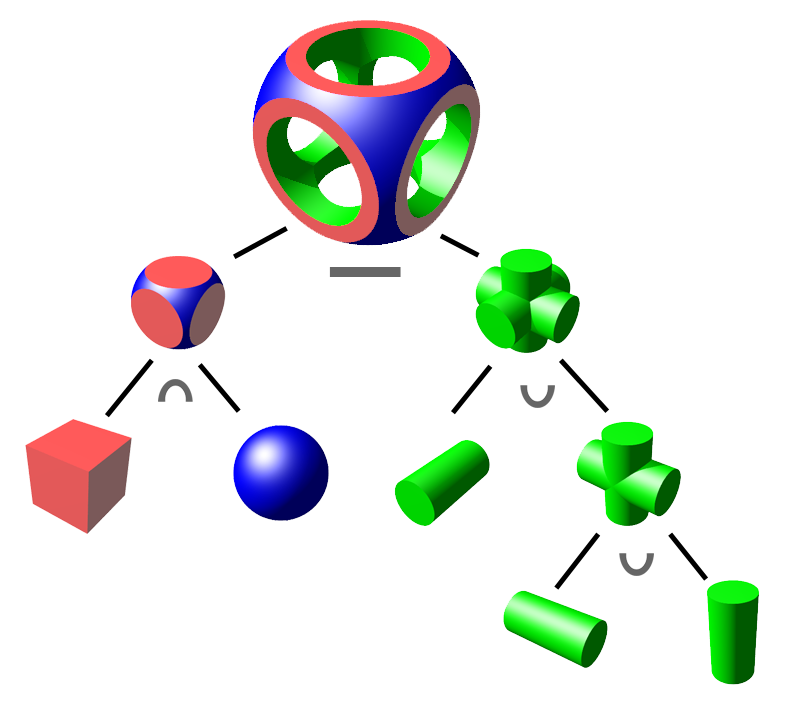
\includegraphics[width=0.5\textwidth]{Pictures/Csg_tree.png}
\caption{CSG object tree, figure taken from \cite{WikipediaCSG}}
\label{fig:csg_tree}
\end{figure}
One way of representing a geometry in CAD is the approach of \emph{constructive solid geometry}. The basic idea is to start from a set of primitives, e.g. a sphere, cylinder and cube. Basic Boolean operations link these primitives towards a complex geometry. This procedure can be seen in figure \ref{fig:csg_tree}.

Key advantages of this format is the precise representation using very little storage memory. However, not all desired forms can be represented by CSG and hence, a second type of geometry description is needed. 
\subsubsection{Boundary representation}
A different kind of modelling approach is the so-called \emph{boundary representation}. Instead of storing the geometry information at every single point, BREP formats only save the boundary surface of the body. The interior is assumed to be uniformly filled. Especially in complex geometries, this approach simplifies the model to such an extent, that the amount of data becomes much easier to handle. Surfaces can then be for example stored as a set of triangles (as in STL files, see \autoref{subsub:STL}) or in NURBS patches (see \autoref{sec:NURBS}).
Furthermore, holes in the body are possible by saving the surface normal of the respective boundary. 

By the boundary representation arbitrary geometries can be created. While the data sizes are commonly larger than in CSG representation, BREP files are usually easier to work with. One also has to keep in mind, that non-physical geometries can result from BREP formats through a not closed surface.
\subsection{Data exchange interfaces}
CAD software programs usually use their own data formats; in order to exchange models standardized interface formats have been developed. Geometric models are compressed to certain geometry descriptions; transferring additional information, such as material properties or manufacturing information, is in general a difficult task and in some exchange file formats even prohibited. A few common exchange file types are described below.
\subsubsection{STL file format} \label{subsub:STL}
The STL (from \emph{ST}ereo\emph{L}ithography) file format describes the model only by its boundary and is thus a BREP format. Because of only taking this into account, only geometric information can be transferred. 

The idea behind the STL files is simple: the geometric model is discretized into a cloud of points. Sets of three vertices form a triangle; hence, a connected surface of triangles emerges which describes the geometry. This procedure is shown in \autoref{fig:STL} for a two dimensional circle.  
\begin{figure}
\centering
   \scalebox{0.4}{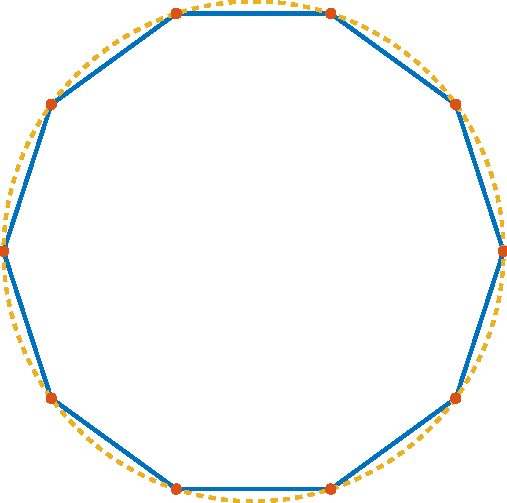
\includegraphics{Pictures/STL.pdf}}\\
   \caption{STL discretization for a circle, self-made in MATLAB}
   \label{fig:STL}
\end{figure}
The aforementioned triangles boil down to lines in two dimensions. The advantages and disadvantages of this approach become clear: It can be applied to an arbitrary geometry, but accuracy causes difficulties. In order to transfer high precision geometries many vertices are necessary. This will result in big files; nevertheless, a precise circle can never be represented. 

ASCII STL files begin with a name and the data on the triangles is constructed as follows: 
\begin{itemize}
\item a facet normal pointing outward
\item a sequence of vertex coordinates
\end{itemize}
Note that no additional information such as material properties are transferred through STL files \cite{STL}.
\subsubsection{STEP file format}
To overcome issues of insufficient precision also more elaborate exchange formats exist; these save e.g. a circle as a parameter where no discretization step is involved. Also, the possibility of passing additional parameter information (e.g. density, manufacturing information) is required by certain users. Popular file types that offer these two functionalities are STEP and IGES files. 

The STEP file format is a newly developed CAD data exchange standard and documented in the ISO 10303 norm. On the contrary to STL files it uses a combination of CSG and BREP to store the geometry. Additional information (e.g. density) are passed through attribute sets that are stored besides geometry instances (e.g. a circle). A key disadvantage, however, is that STEP files carry much redundant information \cite{STL}.
\subsubsection{IGES file format}
 The Initial Graphics Exchange Specification (IGES) is an American 
National Standard since 1981 to exchange graphics information. Similar to the STEP format it uses a combination of CSG and BREP for the geometry representation. Instead of storing a set of manufacturing information as done in the STEP file, the IGES is build only to exchange graphics information. For example, the step file transfers a physical density information; in the IGES format the only additional parameter store node coloring information. Consequentially, IGES file sizes are significantly smaller compared to the STEP file format.

The IGES file format contains five different sections: a \emph{Start}, \emph{Global}, \emph{Directory Entry}, \emph{Parameter Data} and \emph{Terminate} section. The \emph{Start} and \emph{Global} section are used for naming and part information. In the \emph{Directory Entry} section additional information like the node color is saved. The \emph{Parameter Data} section is used for storing the coordinate points; the \emph{Terminate} section signals the end of the file \cite{sarcarCAD}.


\section{Topology Optimisation}
\label{sec:TopOpt}
%how the algorithms work, maybe what it can be used for
\section{Topology Optimisation}
\label{sec:TopOpt}
\emph{Topology optimization} describes the process of finding the optimal distribution of a limited amount of material for a given area or volume based on a predefined constraint/minimization problem. Possible optimization goals are for example \cite{Hunter2009}:
\begin{itemize}
\item \textbf{Minimum compliance}, in which one seeks to find the optimal distribution of material that returns the stiffest possible structure. The structure is thereby subjected to loads (forces) and supports (boundary conditions). By maximizing the stiffness, the compliance is minimized. This is also analogous to minimizing the stress energy stored by the applied loads.
\item \textbf{Heat conduction}, where one tries to optimize the domain of a conductive material with respect to conductivity for the purpose of heat transfer. This maximization problem is the same as minimizing the temperature gradient over the domain --- a poor conductor will create a large gradient.
\item \textbf{Mechanism synthesis}, where the objective is to obtain a device that can convert an input displacement in one location to an output displacement in another location. Thus, one hereby seeks the optimal design which maximizes the output force for a given input, or respectively, minimizes the input force for a given output.
\end{itemize}


As one can already imagine by this short list of optimization goals, topology optimization has a wide field of possible applications. Hence, it has become a well established technology used by engineers in the fields of aeronautics, civil, materials, mechanical and structural optimization. Furthermore, due to the rising significance of additive manufacturing techniques in industry, the realisation of complex optimized designs is now much easier \cite{Yang1995}.
For the rest of this section, and the rest of the document, we will concentrate on the \emph{Minimum compliance} problem. Note however, that almost all parts in the \emph{CAD-Integrated Topology Optimization} tool could just as well be applied to any other topology optimization problem. 

\subsection{Minimum compliance: Problem formulation}
\label{subsec:TopOpTheory}
\begin{figure}
\centering
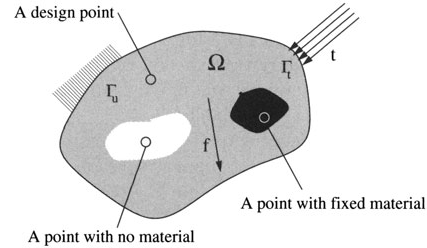
\includegraphics[width=0.6\textwidth]{Pictures/TopOp/design_domain.png}
\caption{The reference domain $\Omega$ for the minimum compliance problem. The problem is formulated such that for a set of external loads $t$ on boundaries $\lambda_t$, body forces $f$ and a set of fixed support points $\lambda_u$, the material distribution within $\Omega$ is such that the stiffness with regards to these loads and forces is maximal and the energy stored by the application of those forces is minimal. The problem also allows defining areas which either cannot or must be filled with material. Figure taken from \cite{bendsoe2003topology}.}
\label{fig:topOpRefDomain}
\end{figure}
In order to constrain the resulting structure as little as possible, the formulation of the topology optimization problem is generally given as follows: for a given set of external fixture points, external loads and/or body forces, the distribution of material within the reference domain should be found such that the structure has maximum stiffness. This is obtained when the structure has the minimum energy stored by external work for the applied forces. The problem is also usually formed to allow for regions in the domain to be specified as filled or empty of material (see \autoref{fig:topOpRefDomain}). 

The formulation allows the problem to be cast as finding a displacement field $u$ and a stiffness tensor field $E$ that is in equilibrium with the applied loads, and that minimizes the external work done by these external loads do to reach that equilibrium. 

\subsection{Physical and mathematical simplifications}
To turn this into a more tractable mathematical problem, a few physical assumptions are also typically made: the material be isotropic and linearly elastic. From the assumptions of isotropy and linear elasticity of the material, the stiffness field becomes a constant of the material, defined where there is material in the domain.

The problem is also easy to cast into a weak form. First of all, we compute the integrated internal virtual work and external work. The former is the work of deforming the elastic material from equilibrium by an admissible displacement. The latter is done by the loads and forces to bring out this displacement. Having computed these, we set them equal to one another in order to conserve energy. As a result we obtain an equation that relates the equilibrium displacement, stiffness tensor, and the forces and loads. We then cast this into the weak form, which can be solved using Finite Element Methods (FEM). These can also incorporate the calculation of the external work done.

\subsection{Solid Isotropic Material with Penalization (SIMP)}
As described in the previous section, we aim to minimise the external work done by looking at different material distributions. However, the usual problem of finding an optimum arises: the search space is vast. After discretising the domain with FEM, the possibilities of where to put material at least are not infinite --- but they still grow exponentially with the number of elements; hence, trying out one-by-one is not going to prove efficient. One popular way of recasting the problem to allow for easier solving is the SIMP model. Here, instead of either being present or not at a point, the material presence can take a continuous set of values between one and zero. The total final volume is then obtained and fixed by integrating this presence variable over the domain, instead of constraining the allowed occupied space. This allows for the interpretation as some kind of density.

In order to still obtain topologies where material is predominant in certain areas --- of densities one, with the rest being empty at densities close to zero --- a "penalty" is applied to the intermediate values. This is effected by raising the density to a power $> 1$ in the elastic energy calculation, but not in the volume calculation. That way, an intermediate density value provides less elastic support, but still "costs" as much volume, and will thus be suboptimal. 

\subsection{Solution and implementation}
\begin{figure}
\centering
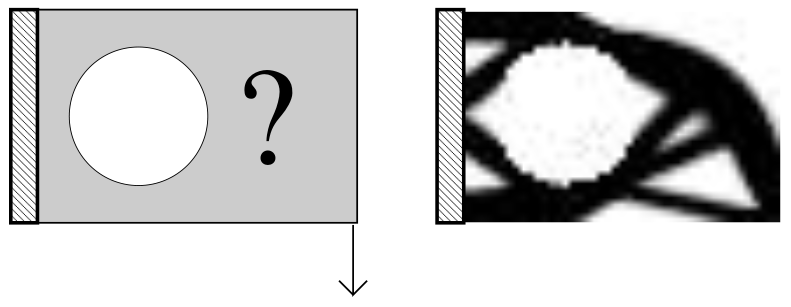
\includegraphics[width=0.6\textwidth]{Pictures/TopOp/Sigmund_cantilever2d.png}
\caption{Topology optimisation of end-loaded cantilever with fixed hole. The optimisation of a loaded cantilever is one of the model problems in topology optimisation, due to its simplicity and its multitude of used solutions throughout the history of engineering. The picture is taken from a known paper by Sigmund \cite{sigmund200199} where a 99-line Matlab code for topology optimisation is introduced.} 
\label{fig:sigmundcantilever}
\end{figure}
In typical implementations, a heuristic iterative scheme is then used for finding a solution. The optimal solution is assumed to have all present parts stressed (as they would otherwise be unnecessary, not providing any support). Thus, at places where the elastic energy is high, material is added if possible, and where it is low, material is likewise removed, with the values "high" and "low" being determined dynamically to keep the total volume constraint. 

This whole scheme is one of the simpler topology optimisation schemes to implement, and has been done so in several pieces of open-source software, including a known 99-line Matlab code by Sigmund \cite{sigmund200199} and ToPy described in \autoref{sec:ToPy}. An example optimised topology is shown in \autoref{fig:sigmundcantilever}. For an extended explanation and discussion, as well as further alternative methods for topology optimisation, the interested reader is referred to \cite{bendsoe2003topology}.



%section moved to implementation
%\section{From CAD to Voxels}
%%SECTION MOVED TO IMPLEMENTATION


%\subsection{Motivation}
%The goal of good design is to find the right balance between a set of parameters, which usually include efficiency, weight and aesthetics. For a long time, this process had been an ardous loop of minute modifications to the product, oscillating between the engineer and the designer. However, with the advent of Topology optimization (see \autoref{sec:TopOpt}) and additive manufacturing, it has been shrunk drastically to an efficient, compact task. In the previous section, we summarized the different ways of representing a design object digitally. On specifying the appropriate loads as boundary conditions on this object, one can choose their favourite topology optimization tool to compute the optimal dimensions and form.


%The main hurdle with most state-of-the-art open source topology optimization tools is their input format, where many of them require input to be specified as a 3-dimensional voxel grid. Presence (or absence) of material in these voxels is defined by a boolean variable, and boundary conditions are imposed on the appropriate locations. An example of voxelized data can be seen in \autoref{fig: voxelOpenCascade}. Since there is a variety of toolboxes available which are able to perform a voxelization of common CAD input files, we did not implement one of our own but rather adapted one of the open source tools. For the implementation we refer to \autoref{sec: CADToVoxels}. %This section describes how we overcame this hurdle of converting CAD representations to voxelized input.
%\begin{figure}
%\centering
%  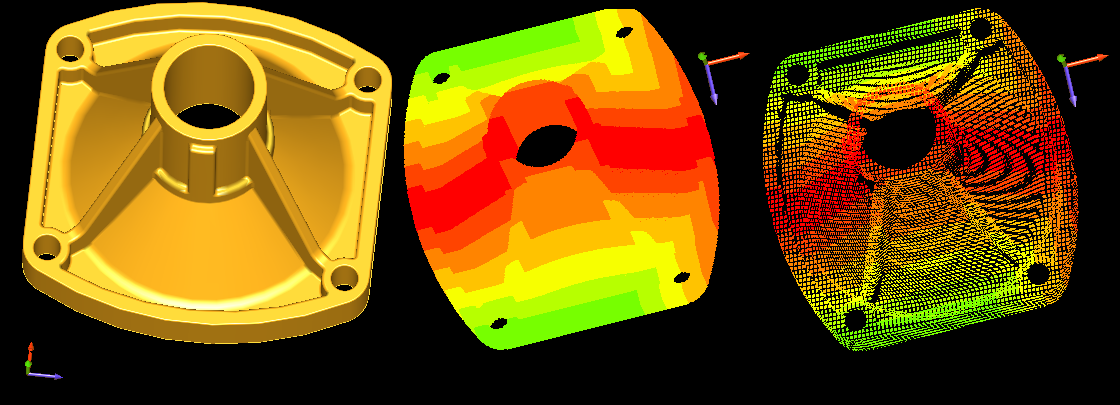
\includegraphics[scale=0.3]{Pictures/CADToVoxel/voxels_wp_image005.png}
%\caption{A shape and its voxel representation. \textem{Leftmost picture}: The original parametrized shape. \textem{Rightmost picture}: The voxel representation. Picture from OpenCascade \cite{OpenCascade}.}
%\label{fig: voxelOpenCascade}
%\end{figure}

 

\section{From Voxels to a surface representation}
\label{sec:surfaceBackg}
%BEGIN JC
\subsection{Isosurface Contouring}
Now when the optimized voxel data was obtained, the next step is to generate a \emph{mesh based
geometry}. It will be useful in the further NURBS implementation. In order to achieve it, the
data will be represented by a contour of a smooth function, rendering an isosurface. The
isosurface allows to visualize Scalar Volumetric Data in 3D. It furthermore permits a mesh
representation of the volume data. The mesh can be composed of triangles or quads, according
to the algorithm used. There are two main approaches to solve this problem, the most
famous one is Marching Cubes.

\begin{figure}
\centering
   \scalebox{0.8}{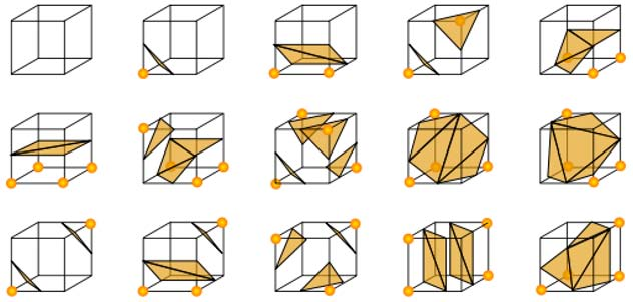
\includegraphics{Pictures/cubes.pdf}}\\
   \caption{Basis cases of Marching Cubes}
\end{figure}

\subsubsection{Marching Cubes} 

This algorithm takes as an input a regular volumetric data set and extracts a polygonal mesh. It
divides the space into cubes, which are defined by the volume information. Each cube has scalar
information on its vertices, the value is equal or above a marked isovalue. Therefore each of the
eight vertices of a cube can be marked or unmarked. According to these values vertices are drawn
on the edges of the cube at calculated points with the use of interpolation. A cube that contains
an edge is called active. Non active cubes are not further considered in the algorithm.

By connecting the vertices we obtain a polygon on each cube. There are 256 possible scenarios,
but most of them are just reflections or rotationally symmetric cases of each other. Therefore
there are 15 base cases which represent all the possibilities of the marching cubes (Figure 2.1). 
The original algorithm presents two main problems. Firstly it does not guarantee neither
correctness nor topological consistency, which means that holes may appear on the surface due
to inaccurate base case selection. The second problem is ambiguity, which appears when two
base cases are possible and the algorithm chooses the incorrect one. These cases can be grouped
into face ambiguities and internal ambiguities. There are many extended Marching Cubes
algorithms that tackle the problems of the original one, getting rid of the ambiguities and
providing correctness.

\subsubsection{Dual Contouring}
The idea of this algorithm is similar to Marching Cubes, but instead of generating vertices on the
edges of the cubes, it locates them inside the cube. Figure 2.5 shows the basic differences in both approaches.
The vertices associated with the four contigous cubes are joined and form a quad. The question now is
which place inside the cube is the ideal one to insert each vertex. Different dual algorithms are classified 
according to the answer for this question. Dual contouring generates a vertex positioned at the minimizer of a
quadratic function which depends on the intersection points and normals. Therefore the method needs Hermite 
data to work with.
\begin{equation*}
E(x)= x^TA^TAx-2x^TA^Tb+b^Tb
\end{equation*}
Where \textit{A} is a matrix whose rows are the normals and \textit{b} is a vector whose entries are the product of normals and intersection points. To solve this system, a nummerical treatement is needed. As proposed in [1] the best approach is to compute the
SVD decomposition of \textit{A} and form the pseudo-inverse by truncating its small singular values. 
%1=Dual Contouring of HErmite DAta


The main advantage of this method over MC is the adquisition of better aspect ratios. On the other hand the need of Hermite Data
represents a disadvantage. Furthermore there is no open source algorithm that implements the Dual Contouring scheme.


\subsection{The VTK Toolbox}
\subsubsection{Installing VTK}
VTK was installed using the Linux platform, for it to be successfully implemented a gcc compiler
must be already on the machine. VTK offers the possibility to use Python, TLC or C++ for
development. VTK toolbox is actually a C++ library, which is implemented in other languages. We
decided to continue the project with C++ since it gives the possibility to explore the original code.
A few dependency problems were encountered, nevertheless they were easy to track back. If any
problems were to be found at installation time, please refer to the VTK Wiki where the procedure
is explained step by step.

\begin{figure}
\centering
   \scalebox{0.35}{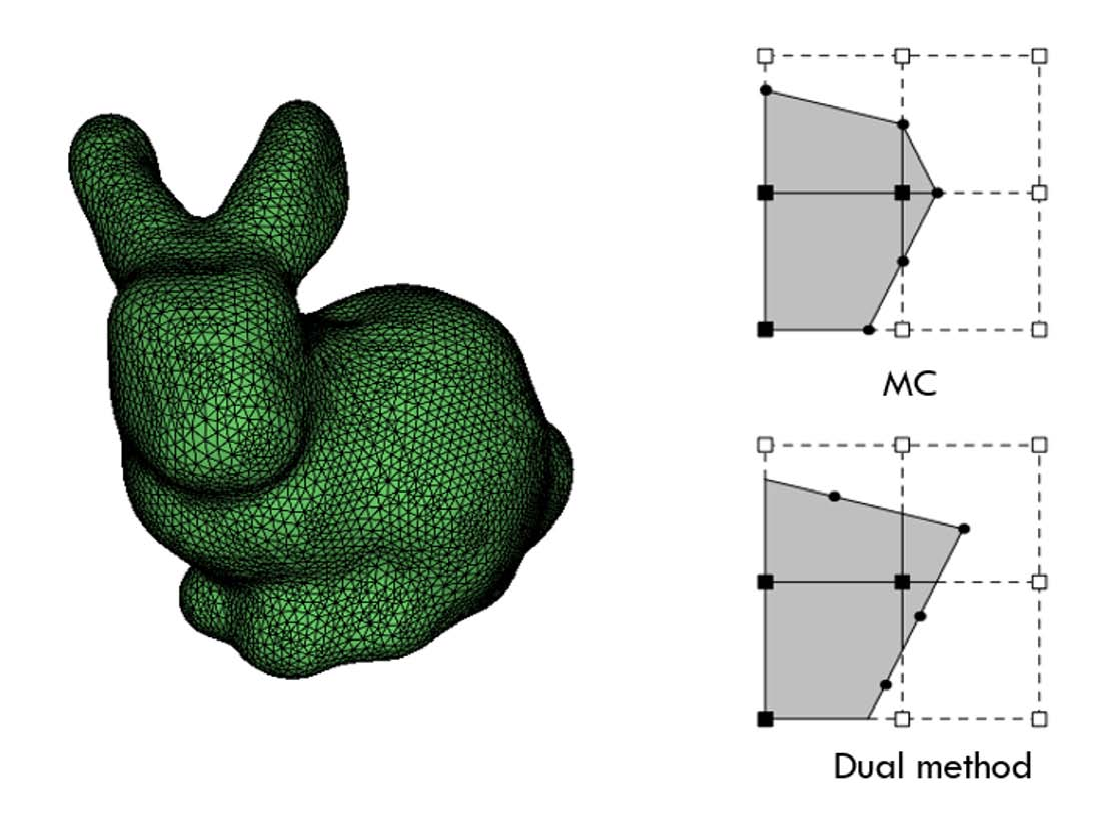
\includegraphics{Pictures/bunny_MC.pdf}}\\
   \caption{\textit{Right:} The famous Standford Bunny. \textit{Left:} Main difference between MC and Dual methods }
\end{figure}

\subsubsection{Implementing the VTK Classes}
The VTK toolbox was used in order to implement the algorithms on our optimized data. It is a heavily object
oriented toolbox. Our first approach was to use the built in Marching Cubes algorithm,
nevertheless it did not work with our unstructured grid data. It just works for ImageData and
PolyData . For structured and unstructured grids the tool to render the isosurface is the contour
Filter tool. Unfortunately the documentation does not present which algorithm the tool uses. It
can be inferred that it is an extended Marching cube algorithm.

The Contour Filtering seemed to work fine but the visualization of our data was still not possible
and an intermediate step was needed. We used the Implicit Modelling tool which is a filter that
computes the distance from the input geometry to the points of an output structured point set.
This distance function can then be "contoured" to generate new, offset surfaces from the original
geometry. It finally allowed visualization but it created one problem. Holes are lost in
the process.

\begin{figure}
\centering
   \scalebox{0.4}{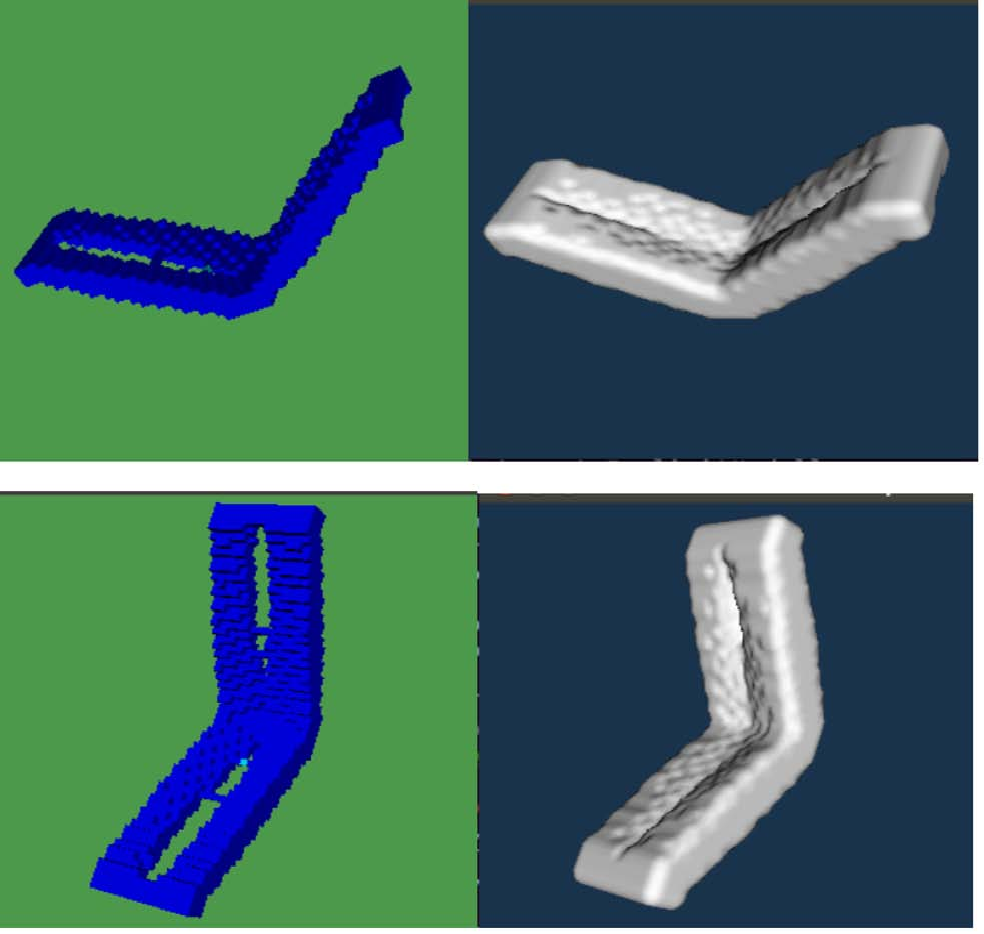
\includegraphics{Pictures/contouring.pdf}}\\
   \caption{Contour Filtering tool after Implicit Modelling}
\end{figure}

A further idea to solve this problem is to convert at the first step the volume data into point data
and only then present it to the Contour Filtering Tool. This will be implemented in the next
milestone.

The next step was to create a coarser mesh from the fine one. The triangles that represent the
isosurface can be reduced with the Decimation tool. A smoothing step is necessary in between
to get the new connections right. The top part of figure [2] shows a 50 \% reduction of the
triangles, a noticeable difference can not be perceived. On the lower part a 90 \% reduction is
obtained, it is nevertheless still difficult to see a difference. Triangle meshes can be easily
coarsened since there are many open source algorithms that simplify the triangles. VTK has the
decimation tool which works for 3D triangle data.

\begin{figure}
\centering
   \scalebox{0.4}{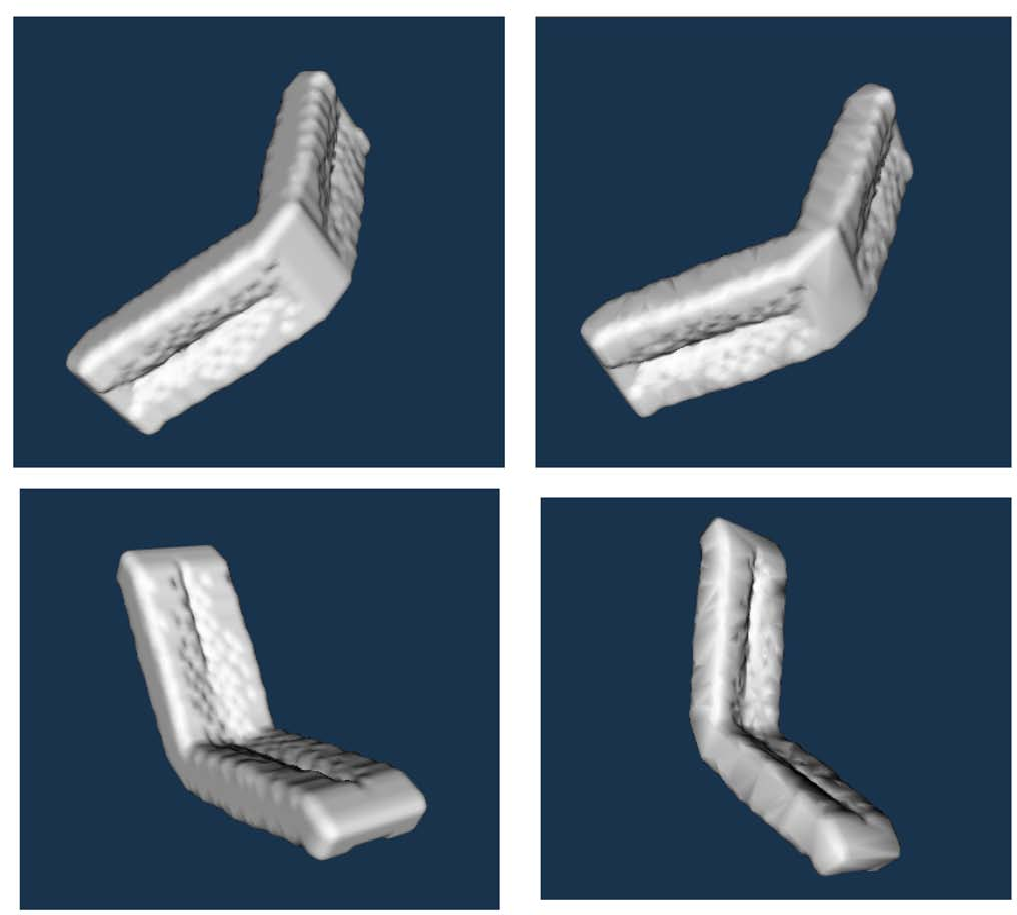
\includegraphics{Pictures/Decimation.pdf}}\\
   \caption{Decimation of triangles. \textit{Top:} 50\% \textit{Lower:}90\%}
\end{figure}

\subsection{The Long Road to NURBS}
There are two possible roads to go from the voxel data to the NURBS representation.
\subsubsection{Quad Contouring}
This approach uses the dual contouring algorithm as first step in order to obtain a quad mesh
representation from the voxel data. The first challenge is to implement correctly the algorithm
with the ideas presented in [1]. The original marching cubes algorithm is
implemented in VTK but the source code is not public, therefore not only an extension
of it is needed, but a full implementation. Once this first step is done, the quads will be chosen for the
NURBS parametrization. A second step considers multiple smaller quads which have to be
combined into one larger patch. This is another challenge, since the remeshing of quad meshes
is not as straight forward as with the triangles. Different approaches have been taken in order to
achieve this coarsening. In [2] an incremental and greedy approach, which is based on local operations only, is presented. It depicts an iterative process which performs local optimizing, coarsening and smoothing operations. Another approaches, like
the one presented in [3] uses smooth harmonic scalar fields to simplify the mesh.
%2= “Practical quad mesh simplification”
%3= “Harmonic Functions for Quadrilateral Remeshing of Arbitrary Manifolds”


\subsubsection{Multiresolution Analysis of Arbitrary Meshes}
With this approach there is no need to apply a Dual Contouring algorithm, since it takes as
beginning data the triangles from the Marching Cubes. The main concepts are shown in the paper
of the same name [4]. It mainly takes a series of intermediate steps which permits a parametrization of data. It includes a partitioning scheme based on the ideas of the Voronoi Diagrams and Delaunay triangulations. Large patches or quads are obtained with this method. Further discussion on this approach is explained in the following section.

%4=reference to MAAM, a.k.a Benni's favorite paper!

Both approaches have not been implemented in open source documentation, therefore it will be
a long road to achieve what is required. For the first part the second
road was chosen and in case it leads to a dead end, the first way will be taken into consideration.

%END JC

\section{From a surface representation to NURBS}
\label{sec:NURBS}
\subsection{Parametric curves}
\todo{add thing about control points in description and possibly names, because they're kinda important}
%As mentioned in the Introduction, the main challenge of our project is to convert the mesh based geometry, obtained on a previous step, back to CAD representation. 
Parametrised geometries are often given in terms of \emph{Non-Uniform Rational B-Spline} (NURBS) curve patches (see for example, documentation of FreeCAD software \cite{FreeCAD}). 
To define NURBS from a mathematical standpoint, we first define so-called \emph{Bezier curves} and use them later for the definition of NURBS. For these two sections, we refer to \cite{farin2002handbook} for a more in-depth introduction and further material. 
\subsubsection{Bezier Curves}
A Bezier curve is a \textit{parametric} curve, which is often used for producing a smooth approximation of a given set of data points.
 
An analytical expression for the Bezier curve parametrized by the variable $u$ is given by:
\begin{equation*}
\vec{B}(u)=\sum\limits_{i=0}^n b_i^n(u) \vec{P}_i
\end{equation*}
where $\vec{P}_i$ is the $i^{\text{th}}$ control point, $i\in0,1, \dots ,n$ ($n+1$ control points in total), and
\begin{equation*}
b_i^n(u)=\binom{n}{i}(1-u)^{(n-i)}u^i
\end{equation*}
with $\binom{n}{i}$ being a binomial coefficient, is the $i^{\text{th}}$ \emph{Bernstein polynomial} (see \cite{lorentz2012bernstein}) of degree $n$.

Additionally to the expression with the Bernstein polynomials, one can use a recursion formula (so-called \emph{de Casteljau Algorithm}) for the construction of the Bezier curve, which we will not cover here.

Analogically to Bezier curves, but with $n\cdot m$ points $\vec{P}_{i,j}$,
one can define a \textit{Bezier surface}, given by the analytical expression
\begin{equation*}
\vec{S}(u,v)=\sum\limits_{i=0}^n \sum\limits_{j=0}^m b_i^n(u) b_j^m(v) \vec{P}_{i,j}
\end{equation*}
\\
Note that Bezier curves \todo{higher-order only?} and surfaces may be unstable --- minor changes in control points might lead to major global changes.


\subsubsection{NURBS basis functions}
\todo[inline]{rename subsubsection and name that Bezier curves are subset of NURBS}
Extending the idea described in previous section, one could use \emph{B-spline basis functions} (see below) instead of the Bernstein polynomial basis.

Unlike with Bezier curves, for the B-splines a parameter domain is subdivided by so-called \textit{knots}. For the one-dimensional parameter domain $[u_{0}, u_{m}]$, the \textit{knot vector} will be given by $u_{0} \leq u_{1} \leq ... \leq u_{m}$. In most cases $u_{0} = 0, u_{m} = 1$ is chosen, so that we get the unit interval for our parameter values. For the case of NURBS, the knots $u_{0},..., u_{m}$ need not be equidistant --- hence the Non-Uniform in the beginning NU of NURBS.

Given a knot vector $[u_{0}, u_{m}]$ and a degree of B-spline $p$, the $i$-th B-spline basis function is then defined recursively as follows:
\begin{equation}
N_{i,0}(u) =  \begin{cases} 1, & \mbox{if } u_{i} \leq u < u_{i+1} \\ 0, & \mbox{otherwise } \end{cases}
\end{equation} 
\begin{equation}
N_{i,p}(u) = \frac{u - u_{i}}{u_{i+p} - u_{i}}N_{i, p-1}(u)  + \frac{u_{i+p+1}-u}{u_{i+p+1} - u_{i+1}}N_{i+1, p-1}(u)
\end{equation}
For $p=0$ we get just step functions, and $p=1$ familiar hat functions, whereas the quadratic basis functions look more complicated (\autoref{fig:bsplineBases}).
\begin{figure}
\centering
\begin{subfigure}[B-spline basis for $p=0$]{
  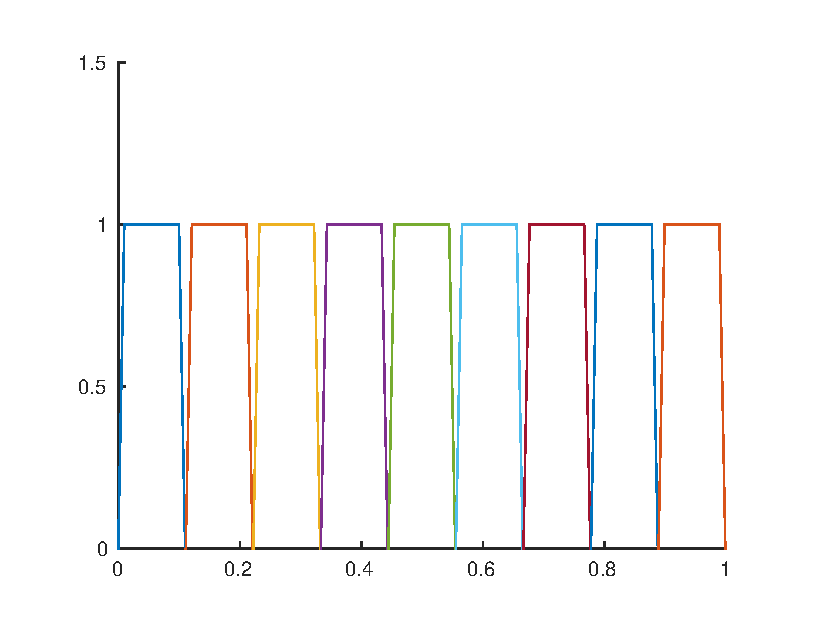
\includegraphics[width=.3\linewidth]{basis_constant.eps}}
  \label{fig:bspline_basis_constant}
\end{subfigure}%
\begin{subfigure}[B-spline basis for $p=1$]{
  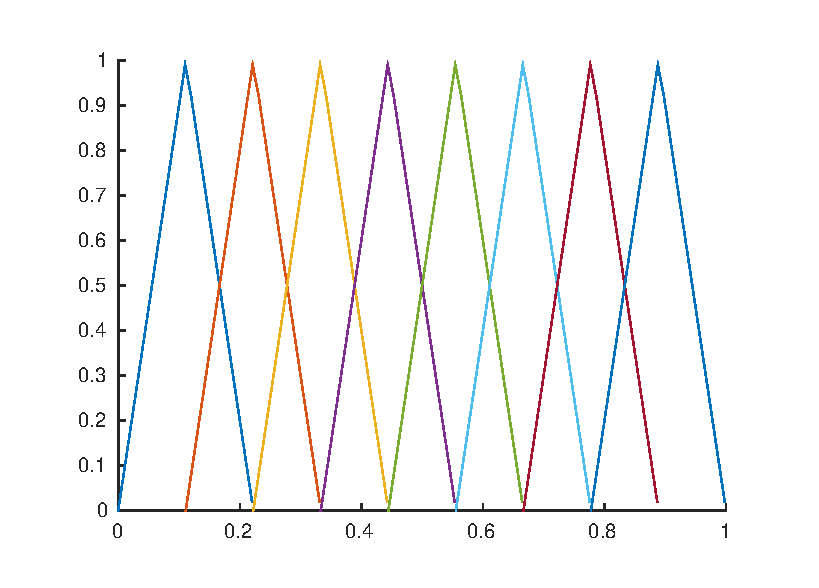
\includegraphics[width=.3\linewidth]{basis_linear.eps}}
  \label{fig:bspline_basis_linear}
\end{subfigure}
\begin{subfigure}[B-spline basis for $p=2$]{
  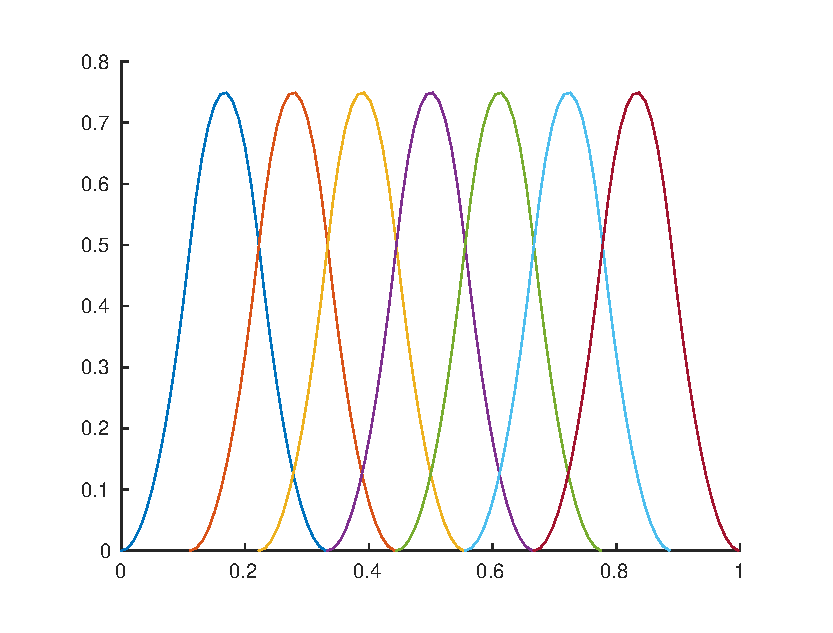
\includegraphics[width=.3\linewidth]{basis_quadratic.eps}}
  \label{fig:lognorm_quadratic}
\end{subfigure}
\caption{B-spline basis functions, of degree $p=0$ (left), $p=1$ (middle) and $p=2$ (right).}
\label{fig:bsplineBases}
\end{figure}


By giving each of these basis functions a weight $\omega_i$ and normalizing them at each point by dividing by the total sum, we get the rational basis functions. Writing them out explicitly, in terms of B-spline basis functions $N_{i,p}$, the $n^{\text{th}}$-degree NURBS curve with $k$ control points $P_i$ is finally given by:
\begin{equation}
C(u) = \frac{\sum_{i=1}^{k}N_{i,n}\omega_{i}P_{i}}{\sum_{i=1}^{k}N_{i,n}\omega_{i}}.
\end{equation}

B-splines are have the following properties, which are useful for our problem:
\begin{itemize}
\item Degree $n$ and number of control points $\vec{P}_{i\cdots m}$ are independent.
\item B-Splines only change locally (depending on the degree $n$) when a control point is changed.
\end{itemize}

Analogically to the Bezier curve surfaces, one can define B-spline or NURBS surfaces. For more information about NURBS see \cite{farin1999nurbs}.
\subsection{Peters' Scheme for $G^1$ B{\'e}zier Surface Reconstruction}
\label{subsec:peters}
Although the process of generating a NURBS surface may seem trivial (placing the control points near the desired surface location), getting it to assume a specified shape can be quite a task. Generating a topology more complex than a torus \todointern{possible reference to figure above} requires several NURBS surfaces joined together. Thus, one needs to fulfil certain requirements in order for these surfaces to remain connected. For simple surface continuity ($C^0$), it is enough that the control points and knots on the edges of the two patches are the same, since then on both edges the surface follows a 1D--NURBS-curve from these points and knots. Smooth surfaces require higher-order continuity, which creates much more complex requirements. Several schemes have been created to automate such tasks.

The approach sometimes referred to as \emph{surface splines} or \emph{G-splines} \cite{eck1996automatic} solves the task of generating a smooth surface by starting from a \emph{control mesh} $\petersControlMesh$ of points, and computes B{\'e}zier surfaces by setting their control points to be linear combinations of the points in $\petersControlMesh$. The coefficients are determined such that the resulting surfaces will be \emph{tangent plane continous}, or $G^1$, or other desired degrees of smoothness.

One such scheme is the scheme of Peters, described in \cite{peters1992constructing}, which starts from an unstructured mesh of polygonal faces, and creates a $G^1$--continous surface from the location and connectivity of its vertices. This means that the normal vector to the plane is countinous, resulting in a smooth surface without sharp corners. The process consists of two steps, described below for a mesh of quadrilateral faces (quads) \cite{eck1996automatic}. However, the scheme could also be applied for a mesh with any mixture of polygons.

\subsubsection{Step 1: Mesh Refinement}
In the first step, the mesh is refined through two iterations of \emph{Doo-Sabin refinement}, as first described in \cite{DooSabin1978subdiv}. This refinement is done by creating new points $\vec{m}_{ref}$ around the vertices $\petersControlMeshVec$ in the control mesh $\petersControlMesh$. One such point is created for every face $f_{\vec{m}}$ that $\petersControlMeshVec$ corners, the new point $\vec{m}_{ref}$ being placed between $\petersControlMeshVec$ and the centroid $\centroidof{f_{\petersControlMeshVec}}$ of the bordering face $f_{\petersControlMeshVec}$ (the centroid of a face being the position of the face's vertices). After having done this for all the points in the control mesh $\petersControlMesh$, we group all the points $\vec{m}_{ref}$ into a new refined mesh $\petersControlMeshRef$. Describing this mathematically for the faces $\petersFaces$, with face ${\hat{f}}\in \petersFaces$ having vertices $V_{\hat{f}}$:

\begin{align}
\petersControlMeshRef =& \left\lbrace \petersControlMeshVec_{ref} \suchthat\petersControlMeshVec_{ref} = \alpha\petersControlMeshVec + (1-\alpha)\centroidof{f} \suchthat f \in \facesof{\petersControlMeshVec} \suchthat \right.
\\ \notag &
 \left. \suchthat \petersControlMeshVec \in \petersControlMesh, \alpha \in (0,1) \right\rbrace
\\
\where \qquad\qquad \centroidof{\hat{f}} =& \; \text{average}\left(\petersControlMeshVec_{\hat{f}}\right)_{\petersControlMeshVec_{\hat{f}} \in \verticesof{\hat{f}}}
\\
\text{and} \qquad\qquad F_{\vec{\hat{m}}} =& \left\lbrace \hat{f} \in \petersFaces \suchthat \vec{\hat{m}} \in \verticesof{\hat{f}}	\right\rbrace
\end{align}
where $\alpha$ is a smoothening parameter, controlling the sharpness of the corners and edges, which we for simplicity set to $1/2$, to get a simple midpoint.

Thus, in every refinement step on an $n$--gon, $n$ vertices are created, giving 4 vertices for a quad in the original control mesh. These are then joined up with the neighbours on the quad to form a smaller quad, and with the neighbouring points from the same vertex on the neighbouring quads, forming a quad along each edge. Around a quad corner, where $n$ quads meet (or $n$ edges in the general case), we instead get an $n$--gon around the corner vertex. After two refinements, we thus get a mesh of vertices $\petersControlMeshDobRef := \petersPatchPoints$ that mainly consists of quads, with possibilities of getting polygons with other number of edges around the vertices of the original mesh $\petersControlMesh$. The mesh and the resulting structure after two subdivisions can be seen in \autoref{fig:petersSubDivide}b.

\begin{figure}
	\centering
	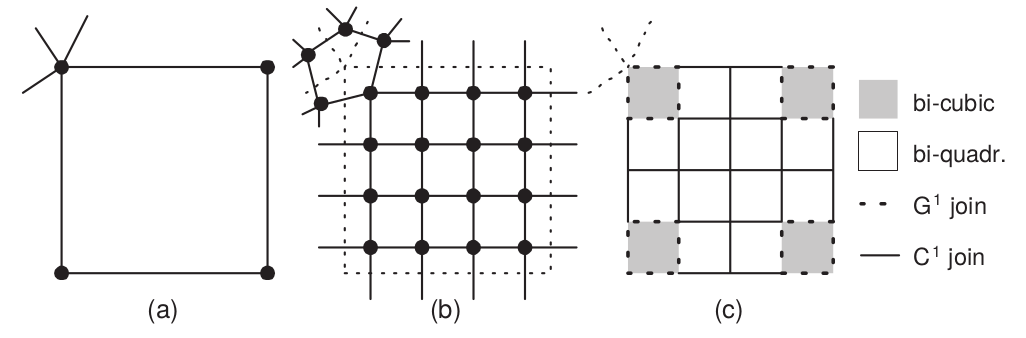
\includegraphics[width = \textwidth]{Pictures/NURBS/petersQuad_to_patches.png}
	\caption{The subdivision step in Peter's scheme. a): A quad in the original mesh, with edges and vertices marked out. Note that there are 5 edges connecting the top-left corner, making this a non-regular mesh corner. b): The mesh resulting from two Doo-Sabin subdivisions, denoted $\petersPatchPoints$ in the text. The mesh is regular, except for around the original mesh corners with other than 4 edges. In the case of the top-left corner, the 5 edges result in a pentagon. c): The resulting \Bez patch structure. The surface is at least $G^1$ continous everywhere. Figure from \cite{eck1996automatic}.}
	\label{fig:petersSubDivide}
\end{figure}

\subsubsection{Step 2: \Bez Patch Creation}
In this step, we create one \Bez patch for every vertex in the double refined mesh $\petersPatchPoints$. 

To begin with, we can recognize that each original quad now has a $4 \times 4$ grid of vertices, where the $4$ vertices along each original quad edge match the $4$ vertices on the neighbouring quad (see \autoref{fig:petersSubDivide}b). From this, we see that most of the cells will be locally in a regular grid, in the sense that it can be seen as the center grid point in a $3\times3$ \todointernal[author=Benni]{which $3\times3$ grid? I thought its $4\times4$...Is it the red grid in Fig. 2.4.3 a)?}two-dimensional structured grid. For illustration, we can look at \autoref{subfig:peterspoints}, where this $4 \times 4$ grid of vertices is marked with black or green crosses. Here, the green crosses illustrate one such local neighbourhood, where the green point in the middle of the darker patch $\petersLocalPatchPointIndices{0,0}$ can be seen as the centre point of the $3 \times 3$ green points $\petersLocalPatchPointIndices{i,j}$, $i,j \in \left \lbrace-1,0,1\right \rbrace$, around it (although the global mesh might look very different further away).% have $8$ local neighbours ($4$ along the edges of the double refined quads, and $4$ along the diagonals of the doubly refined quads). 

Now, for any of these local neighbourhoods of $3\times3$ points $\petersLocalPatchPointIndices{i,j}$, $i,j \in \left \lbrace-1,0,1\right \rbrace$, we can now interpret them as the control points for a biquadratic (that is, second-order) tensor product B-spline surface (meaning with uniform knots). If a neighbouring point is also in a locally regular  $3\times3$ point neighbourhood, we could then extend the B-spline surface to this local neighbourhood by adding them as control points in that direction, using some extra knots. This way, we could build up a network of patches using all the points that are also locally in a regular grid (and their neighbours in their own local $3\times3$ grid). This would results in a $C^1$ continous surface around all vertices where the mesh is locally regular.
%For those cells, we can now create biquadratic tensor splines that meet $G^1$ along the edges and corners; that is, the tensor product of one quadratic spline in one of the regular mesh directions and one in the other.
Now, this surface can also be represented by a network of a biquadratic tensor product \Bez surface patches (see \autoref{fig:petersSubDivide}c for the patch structure), which we will use to describe the whole surface. This means, around a vertex $\petersLocalPatchPointIndices{0,0}$, we create \Bez surface, with $3\times3$ control points for each patch, that we choose to call $\petersLocalBezPointIndices{i,j}$ ($i,j \in \left \lbrace{-1},0,1\right \rbrace$). If we do this, the $3\times3$ \Bez control points $\petersLocalBezPointIndices{i,j}$ will lie at positions in-between the center vertex $\petersLocalPatchPointIndices{0,0}$ and the $3\times3$ local grid vertices $\petersLocalPatchPointIndices{i,j}$, as shown in \cite{peters1992constructing}:
\begin{equation}
\petersLocalBezPointIndices{i,j} = \frac{1}{4}\left(\petersLocalPatchPointIndices{i,j} + \petersLocalPatchPointIndices{i,0} + \petersLocalPatchPointIndices{0,j} + \petersLocalPatchPointIndices{0,0}\right)
\end{equation}
or, writing it out explicitly for $i,j \in \left \lbrace{-1},0,1\right \rbrace$,

\begin{scriptsize}
\begin{align*}
\petersLocalBezPointIndices{{-1},1\phantom{-}} =&\, \frac{1}{4}\left(\petersLocalPatchPointIndices{{-1},1} + \petersLocalPatchPointIndices{{-1},0} + \petersLocalPatchPointIndices{0,1} + \petersLocalPatchPointIndices{0,0}\right)
&
\petersLocalBezPointIndices{0,1\phantom{-}} =&\, \frac{1}{2}\left(\petersLocalPatchPointIndices{0,1} + \petersLocalPatchPointIndices{0,0}\right)
&
\petersLocalBezPointIndices{1,1\phantom{-}} =&\, \frac{1}{4}\left(\petersLocalPatchPointIndices{1,1} + \petersLocalPatchPointIndices{1,0} + \petersLocalPatchPointIndices{0,1} + \petersLocalPatchPointIndices{0,0}\right)
\\
\petersLocalBezPointIndices{{-1},0\phantom{-}} =&\, \frac{1}{2}\left(\petersLocalPatchPointIndices{{-1},0} +  \petersLocalPatchPointIndices{0,0}\right) 
&
\petersLocalBezPointIndices{0,0\phantom{-}} =&\,\phantom{\frac{1}{2}\Bigl(} \petersLocalPatchPointIndices{0,0}\phantom{\Bigr)}
&
\petersLocalBezPointIndices{1,0\phantom{-}} =&\, \frac{1}{2}\left(\petersLocalPatchPointIndices{1,0} + \petersLocalPatchPointIndices{0,0}\right)
\\
\petersLocalBezPointIndices{{-1},{-1}} =&\, \frac{1}{4}\left(\petersLocalPatchPointIndices{{-1},{-1}} + \petersLocalPatchPointIndices{{-1},0} + \petersLocalPatchPointIndices{0,{-1}} + \petersLocalPatchPointIndices{0,0}\right) 
&
\petersLocalBezPointIndices{0,{-1}} =&\, \frac{1}{2}\left(\petersLocalPatchPointIndices{0,{-1}} + \petersLocalPatchPointIndices{0,0}\right)
&
\petersLocalBezPointIndices{1,{-1}} =&\, \frac{1}{4}\left(\petersLocalPatchPointIndices{1,{-1}} + \petersLocalPatchPointIndices{1,0} + \petersLocalPatchPointIndices{0,{-1}} + \petersLocalPatchPointIndices{0,0}\right)
\end{align*}
\end{scriptsize}

\begin{figure}
\begin{center}
\begin{subfigure}[b]{.49\textwidth}
\begin{center}
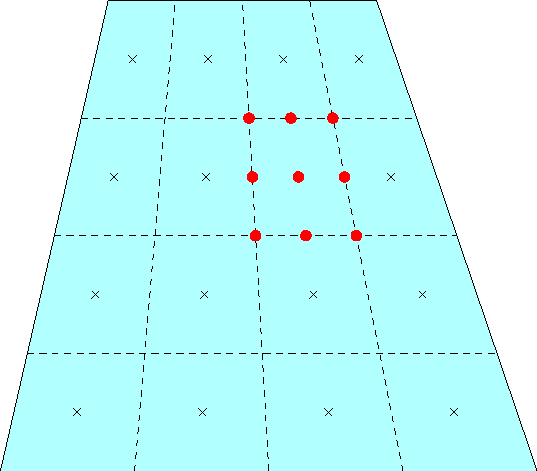
\includegraphics[width=.9\textwidth]{Pictures/NURBS/bezier_points.pdf}
\subcaption{Different points on a quad.}
\label{subfig:peterspoints}
\end{center}
\end{subfigure}
~
\begin{subfigure}[b]{.49\textwidth}
\begin{center}
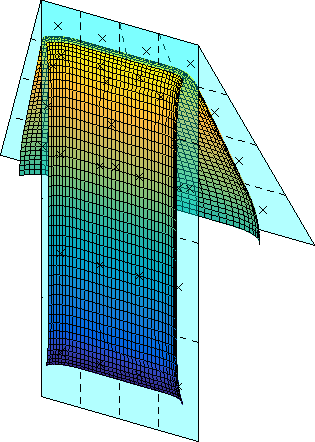
\includegraphics[height=\textwidth]{Pictures/NURBS/bspline_patches.pdf}
\subcaption{Smoothly connected \Bez patches.}
\label{subfig:smoothsurf}
\end{center}
\end{subfigure}
\caption{(\subref{subfig:peterspoints}): The different points used in Peter's scheme. For the quad in the picture with vertices $A,B,C,D$ in $\petersControlMesh$, the refined mesh vertices in $\petersPatchPoints$ created by two Doo-Sabin refinements are marked out with crosses. The extent of each of their \Bez surface patches is also marked on the quad with dotted lines (see \autoref{fig:petersSubDivide}b,c for comparison). Additionally, for the highlighted patch, the tensor product \Bez surface points $\petersLocalBezPointIndices{i,j}$ are marked with red circles, with the corresponding refined mesh points $\petersLocalPatchPointIndices{i,j}$ being the green crosses. (\subref{subfig:smoothsurf}): The resulting smoothly connected surface after creating \Bez surface patches. For visibility, two quads have been cut-out, although the surface is part of a bigger figure. The refined points in $\petersPatchPoints$ are again marked with crosses.}
\label{fig:petersDiags}
\end{center}
\end{figure}

The creation of these different types of points is also illustrated in \autoref{subfig:peterspoints}. 


%as following (see [\todointern[inline]{ref to figure with names on points, EckHoppe or Peters}] for nomenclature):
%%
%\begin{equation}
%
%\end{equation}
%%
To summarize, we have thus just created a surface around all the vertices that are locally in a regular mesh. The exceptions that cannot be placed as such, are now the points residing on the corners of the original quads, since any number of quads may be meeting there.
%This comes from the fact that at quad corners, we may have any number of quads meeting, starting from 3. 
For $n$ quads sharing a corner vertex, the refinement steps will create a polygon with $n$ sides, as mentioned above. If $n\neq4$, the vertices of these corner polygons cannot be placed in a locally regular mesh, and we cannot apply the previous technique -- see for example the upper-left corner of \autoref{fig:petersSubDivide}b.

However, we can still create a \Bez patch which connects smoothly to the locally regular points. To do this, we create a bicubic \Bez patch (of polynomial order 3, one higher than around the regular points, meaning it has $4\times4$ control points) for every vertex in the corner polygon.
We then evaluate how the surface position and normal direction depends on the \Bez control points along all edges of the patches. In order to have a smooth connection, we want these to match, and thus, we can produce constraints for the positions of the \Bez control points.
Since the surfaces are defined at each point as linear combinations of the \Bez control points (which in turn are linear combinations of the vertices in the doubly refined mesh $\petersPatchPoints$), the constraints result in an underdetermined system of linear equations for all the \Bez control points on the bicubic \Bez patches on the vertices in the doubly refined mesh $\petersPatchPoints$.

As the resulting formulae for the locations of the \Bez control points are rather lengthy and complex, we refer to the original paper (ref. \cite{peters1992constructing}). Here, it is also proven that the surfaces have an overall $G^1$ connectivity. A cut-out sample can be seen in \autoref{subfig:smoothsurf}.

To summarize, Peters' scheme is a mathematical algorithm for creating biquadratic and bicubic \Bez patches that join with $G^1$ continuity, from a mesh of polygons. Firstly, a set of refined mesh points is created on each polygon. Then, \Bez control points defining the patches are created as linear combinations of the vertices in this refined mesh. The $G^1$ continuity results from the interpretation of the refined mesh as a regular biquadratic tensor product B-spline surface, and where this is not possible, bicubic \Bez patches are constrained to join smoothly to the surrounding biquadratic patches.
%In this section we will cover the following, referring to \cite{peters1992constructing}:
%\begin{itemize}
%\item How we go from polygonal faces to a set of mesh control points. "patch points", specifying that we're talking about quads, and that we then get 16
%\item That for each of these 16 points, we will make a small B{\'e}zier patch
%\item That if we define the B{\'e}zier control points of these patches in a special way, as described in appendix XYZ \todointern{TODO: create this appendix, or change this to refer to paper for coefficients}, we get a surface that is $G^1$ continous
%\item Maybe describe that we then need for every one of these B{\'e}zier patches the locations of the neighbours
%\item That the location of a point on the surface defined by parameters $\vec{s} = (u,v)$ depends on the B{\'e}zier control points, whose linear dependence on the "patch points" give us coefficients on these "patch points" of the location described by the parameters, as can be seen in \autoref{fig:PetersPoints}
%
%\end{itemize}


%\begin{figure}
%
%\missingfigure{Graphical description of all those different points in Peters' Scheme}
%\label{fig:PetersPoints}
%\caption{The points in Peters' Scheme. As clearly seen in the figure above, this scheme is self-explanatory.}
%\end{figure}



\subsection{Fitting problem}
In order to represent a given line or surface by Bezier curves or surfaces respectively, just as with NURBS, one has to solve a fitting problem. The goal of it is to fit in a parametric curve to the set of given data points. In the case of interest, the given set of points is a mesh, obtained from surface contouring.
\subsubsection{Fitting problem: Bezier curve}
First we want to find a Bezier-curve $\vec{B}_n\left(u\right)$ of degree $n$ which is approximating a given spline $\vec{s}_m\left(u\right)$ defined by $m$ points in a optimal way. For this purpose we want to minimize the L2--error. This leads to the minimization problem
\begin{equation}
\text{find\ } \underset{\vec{B}_n\in \mathbb{B}_n}{\min} \Ltwonorm{\vec{B}_n-\vec{s}_m}.
\end{equation}
Minimizing the L2--norm is equal to minimizing the functional:
\begin{equation}
F(\vec{B}_n)=\int\limits_{u=0}^{u=1} \left(\vec{B}_n-\vec{s}_m\right)^2\du
\end{equation}
Using the variational principle we get the the system of linear equations
\begin{equation}
A a = b
\end{equation}
where $A$ is the matrix of pair-wise scalar products of basis functions (Bernstein polynomials), $b$ is the vector of scalar products of the given spline $s_{m}$ and basis functions and $a$ is a required vector of coefficients for Bezier curve representation.

\subsubsection{Fitting problem (least squares): NURBS}
\todo[inline]{why (least squares) here and not above? is this consistent?}
Although the approach used above showed good results, it appears to be very computationally intensive. Analogically, one could reduce the original problem to a \emph{regression problem}, which allows us to reduce computational costs. Also, to improve the locality of our solution, from now on we are going to use NURBS basis functions with weights $\omega_{j} = 1$ instead of Bezier curves. For this purpose, we adopted an algorithm, provided in \cite{becker2011advanced}:

Let $X^{0}$ be the $n \times 2$ matrix of the given set of points, $N^{p}$ the basis functions of degree $p$ ($n \times (n+p)$ matrix, where $n$ is the number of points), and $P^{0}$ the control points ($(n+p) \times 2$ matrix).

The original problem can be written as:
\begin{equation}
X_{i}^{0} = \sum\limits_{j=1}^{n+p} P_{j}^{0} N_{i,j}^{p}, \quad i \in \{1,..,n\}
\end{equation}
Or, in short:
\begin{equation}
X^{0} = N^{p} P^{0}
\end{equation}
The above system needs to be solved for the unknown $P^{0}$. This can be done numerically, for example through singular value decomposition. 
%part of implementation

\subsubsection{Fitting Problem: Peter's Scheme}
\todo[inline]{insert stuff here}



		
 ---------------------------------------------------------------------------
		%
		% Implementation 
		%
--------------------------------------------------------------------------
		% change chapter/section/part names as pleaseth thee!
%
% possibly later split into software pipeline/nurbs algorithms part!
%\section{Introduction to the software pipeline}
%not written yet

\todo[inline]{comment on the content of this chapter like at the beginning in other chapters}

\todo[inline]{this chapter covers the interfaces and application of the theory from the last chapter}

\section{From \acs{CAD} to Voxels}
\todo[inline]{OpenCascade Class UML diagramm }
\todo[inline]{reading geometries, voxelise to VoxelBoolDS, Writer classes }
\label{sec: CADToVoxels}
One of the hurdles with most state-of-the-art open source topology optimization tools is their input format, where many of them (including ToPy, our topology optimizer of choice) require input to be specified as a 3-dimensional voxel grid. Presence (or absence) of material in these voxels is defined by a boolean variable, and boundary conditions are imposed on the appropriate locations. An example of voxelized data can be seen in \autoref{fig: voxelOpenCascade}. %Since there is a variety of toolboxes available which are able to perform a voxelization of common CAD input files, we did not implement one of our own but rather adapted one of the open source tools. %This section describes how we overcame this hurdle of converting CAD representations to voxelized input.
\begin{figure}
\centering
  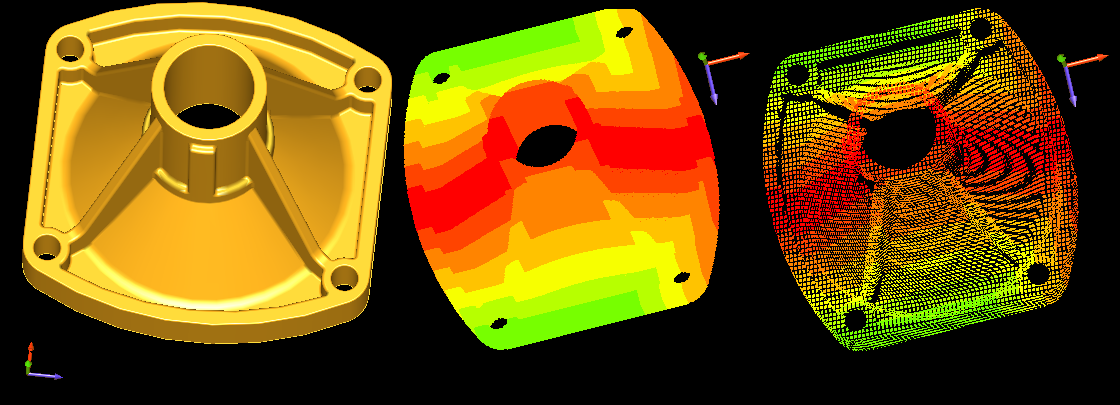
\includegraphics[scale=0.3]{Pictures/CADToVoxel/voxels_wp_image005.png}
\caption{A shape and its voxel representation. \emph{Leftmost picture}: The original parametrized shape. \emph{Rightmost picture}: The voxel representation. Picture from OpenCascade \cite{OpenCascade}.}
\label{fig: voxelOpenCascade}
\end{figure}

\label{sec:CVMLCPP}
In the variety of toolboxes available for voxelization, we decided on the \emph{Common Versatile Multi-purpose Library for C++} (CVMLCPP). This is a collection of mathematical algorithms whose objective is "to eliminate this redundancy by offering high-quality implementations of commonly needed functionality" \cite{CVMLCPP}. The library offers an easy-to-use voxelizer, which we use for conversion of CAD input to a boolean voxel grid.

Another very popular open-source choice is the 3D modeling toolbox is OpenCascade \cite{OpenCascade}, a versatile library with huge amounts of functionality. Although this also offers a voxelizer, we decided that its additional functionality did not justify its disadvantages in size and cumbersome installation requirements on for example a linux system.
\begin{figure}
\centering
\begin{subfigure}{
  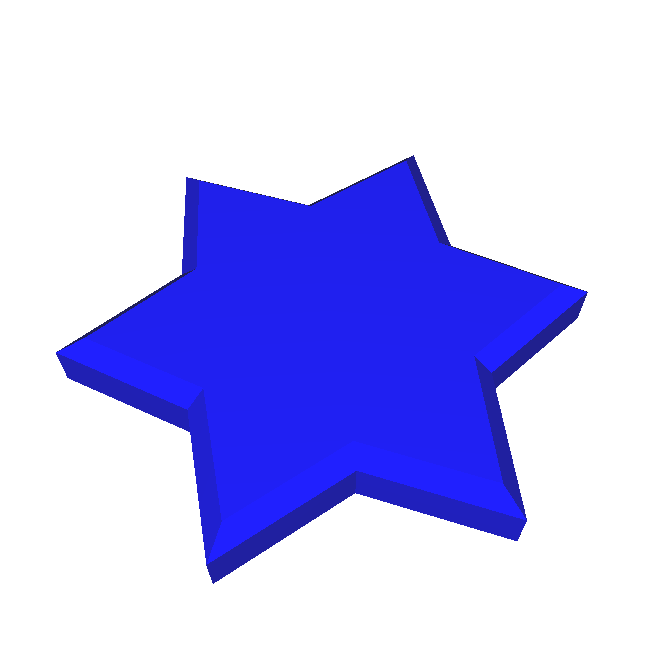
\includegraphics[width=.2\linewidth]{Pictures/STLToVoxels/Star_STL.png}}
\end{subfigure}
\begin{subfigure}{
  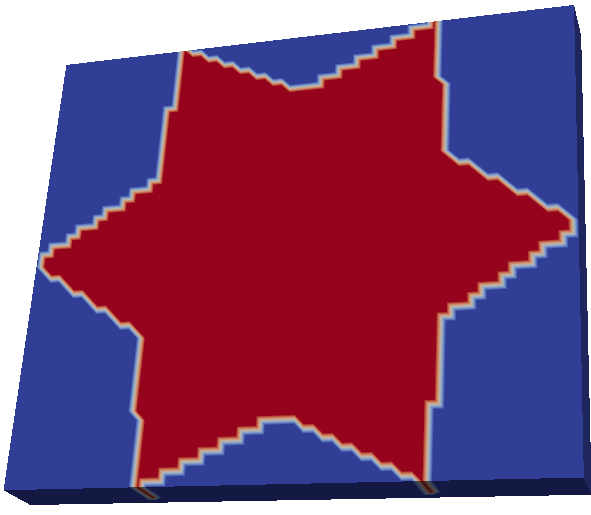
\includegraphics[width=.2\linewidth]{Pictures/STLToVoxels/Star_VTK_Trans.png}}
\end{subfigure}
\caption{The STL geometry of a star (left) and its voxelized form (right) obtained via the CVMLCPP voxelizer, visualized by Paraview \cite{Paraview}.}
\label{fig: voxelizerStar}
\end{figure}

In terms of implementation, the only thing required is the installation of the CVMLCPP library. The voxelizer is then included as a callable binary, that takes STL-file input (\autoref{subsub:STL}) and converts it to a .dat binary file with dimension and voxel information, with specifiable voxel size. An example result of using the voxelizer is shown in \autoref{fig: voxelizerStar}.
 %In the end, to voxelize a file given as .stl-input, we could just call 
%\begin{lstlisting}
%~/Path/To/CVMLCPP/bin/voxelize ./<stl_file>.stl <voxelSize>
%\end{lstlisting}
%where $\mathtt{<voxelSize>}$ is an integer declaring the size of a voxel. 


\section{Topology Optimization}
\label{sec:ToPy}
\todointern[inline]{Severin: Review}
Due to the good range of topology optimization software available, we decided to adapt an open-source topology optimizer to our needs, namely \emph{ToPy}.


ToPy \cite{ToPy} is a python library/program, written by William Hunter and documented in \cite{Hunter2009}, implementing the SIMP model and method described in \autoref{subsec:TopOpTheory}. It is based on the 99-line Matlab code by Sigmund's for minimum compliance \cite{sigmund200199}. The program can optimize the previously named problem types: minimum compliance, heat conduction and mechanism synthesis --- in 2D as well as 3D. It uses highly optimized open source python libraries such as Pysparse \cite{Pysparse} and Numpy \cite{Numpy}, leading to improved speed, porta- and scalability. %The whole program is steered by an input file which-- with the help of the documentation-- is straightforward to use and easy to adapt. %citation on pysparse and numpy


%In terms of our implementation, 
We use ToPy as a black-box topology optimizer. This means, we launch the program with an input file based on our scenario and let ToPy run. Next, as soon as the output is available, we proceed with the next step. The intention is to create separate modules to be able to plug in different solvers later on. In order to specify our input, we wrote an auxiliary program taking a voxelized CAD design provided by OpenCascade as input, outputting a .tpd file with geometry, load and fixture information in the format required by ToPy. 

Results of the topology optimization process can be seen in figure \ref{fig: topyStar}. Here, a star was given as input from a STL-file. We set the voxels in the star's points as fixtures, while we set a load in the middle, in the direction normal to the plane of the star. As can be seen, the optimization process "cuts" away unnecessary material in-between the corners and even in the middle of the material, returning an optimally stiff structure for the chosen remaining volume fraction. 
\begin{figure}
\centering
\begin{subfigure}[c]{.24\linewidth}
\centering
  
\includegraphics[width=\linewidth]{Pictures/TopOp/Star_Optimized0_Trans.png}
\end{subfigure}%
\begin{subfigure}[c]{.24\linewidth}
\centering
  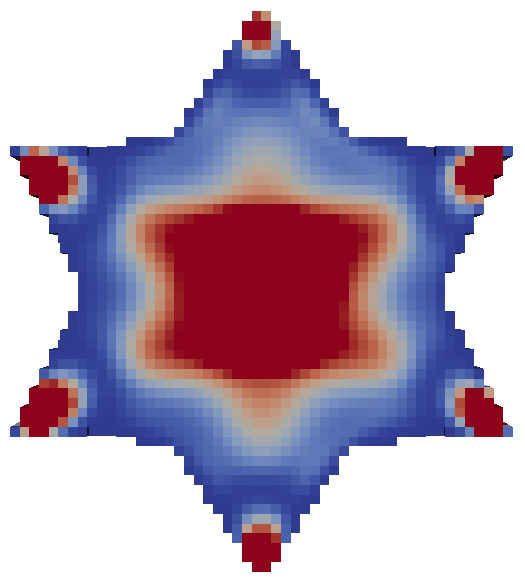
\includegraphics[width=\linewidth]{Pictures/TopOp/Star_Optimized2_Trans.png}
\end{subfigure}
\begin{subfigure}[c]{.24\linewidth}
\centering
  
\includegraphics[width=\linewidth]{Pictures/TopOp/Star_Optimized4_Trans.png}
\end{subfigure}
\begin{subfigure}[c]{.24\linewidth}
\centering
  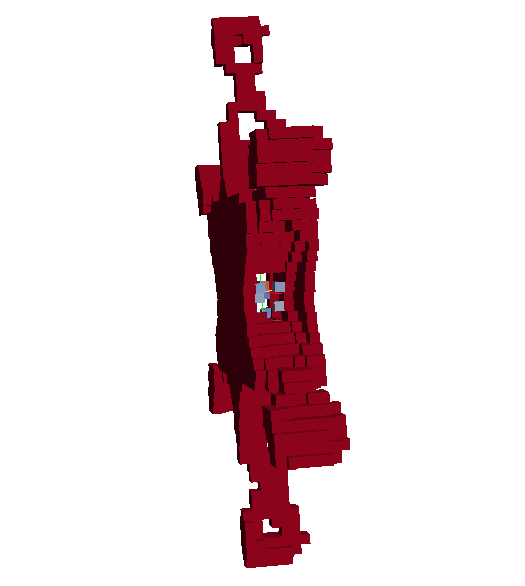
\includegraphics[width=\linewidth]{Pictures/TopOp/Star_Optimized5_Trans.png}
\end{subfigure}
\caption{Topology Optimization by ToPy \cite{ToPy}, with minimum compliance. \emph{From left to right}: increasing number of SIMP iterations until convergence. The star-shaped structure was given by an STL-file which was processed into input readable by ToPy, with fixtures in the corners, and a load in the middle. Throughout the SIMP iterations, one can see how material from the less dense regions (blue) is concentrated into denser regions (red) that carry the load. The last picture gives a rotated view, to illustrate how material has been eliminated even from the inside of the star. } %which volume fraction?
\label{fig: topyStar}
\end{figure}


As was mentioned above, surface extraction is an intermediate step after Topology Optimization and NURBS representation in order to facilitate the conversion. In terms of implementing the surface extraction, we used VTK.

%\subsection{VTK Toolbox}


%The VTK toolbox was used in order to implement the algorithms on our optimized data. It is a heavily object
%oriented toolbox. Our first approach was to use the built in Marching Cubes algorithm,
%nevertheless it did not work with our unstructured grid data. It just works for ImageData and
%PolyData . For structured and unstructured grids the tool to render the isosurface is the \textit{Contour Filter} tool. Unfortunately the documentation does not present which algorithm the tool uses. It
%can be inferred that it is an extended Marching cubes algorithm.

The VTK Toolbox is an open--source tool, providing algorithms for "3D computer graphics, image processing, and visualization" \cite{VTKToolbox}. Among the variety of tools, VTK offers algorithms that allow us to obtain a surface representation from voxel data. Among these algorithms, we could find Marching Cubes, Dual Contouring and also a Decimation method, which is useful for reducing the data size further for the NURBS-representation step.


%\subsection{Implementation}
Since \textit{Marching Cubes} algorithm only works with ImageData and PolyData, it is inapplicable to our case of unstructured grid data. For structured and unstructured grids the tool to render the isosurface is the \textit{Contour Filter} tool. Unfortunately, the documentation does not present which algorithm the tool uses. It can be inferred that it is an extended \textit{Marching Cubes} algorithm.
The \textit{Contour Filtering} works fine but the visualization of our data was still not possible
and an intermediate step was needed. We used the \textit{Implicit Modelling} tool which is a filter that
computes the distance from the input geometry to the points of an output structured point set.
This distance function can then be "contoured" to generate new, offset surfaces from the original
geometry. Although this approach allowed the visualisation, some crucial information was lost. In particular, holes are not represented in the final model.  
%It finally allowed visualization but it created one problem. Holes are lost in
%the process.

\begin{figure}
\centering
   \scalebox{0.4}{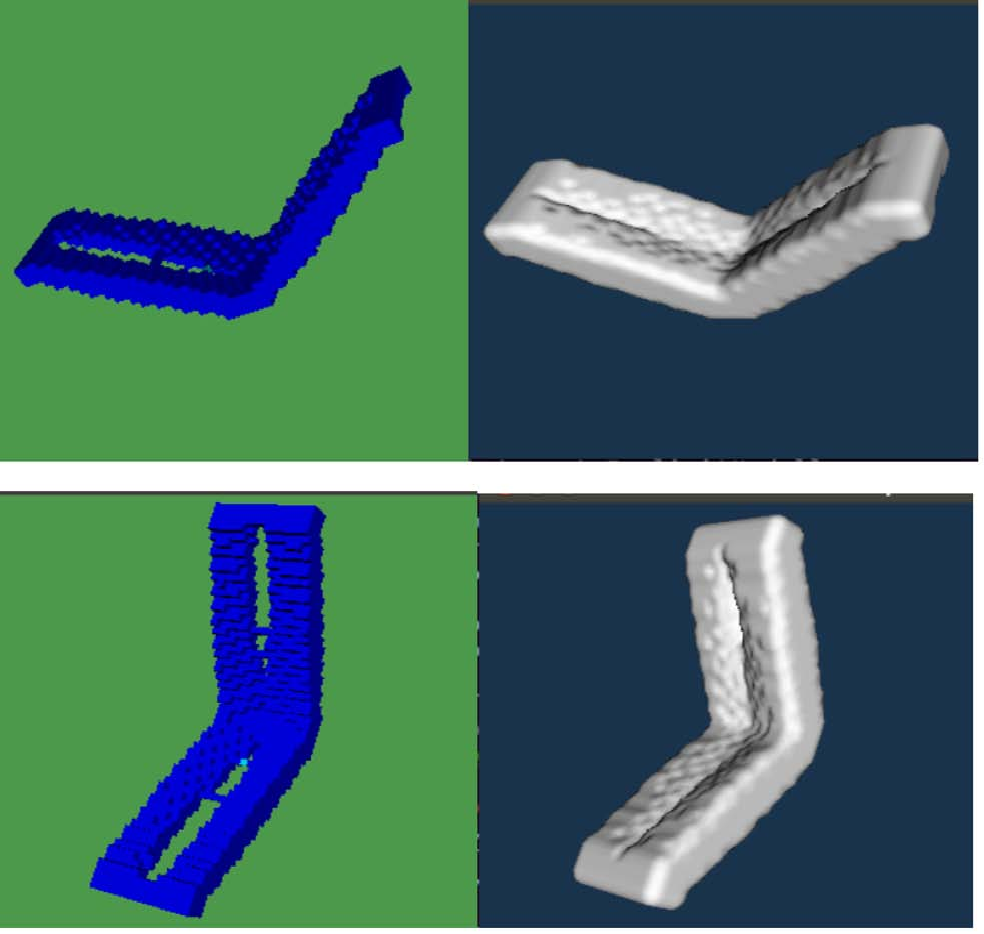
\includegraphics{Pictures/contouring.pdf}}\\
   \caption{Contour Filtering tool after Implicit Modelling}
   \label{fig:contouring}
\end{figure}

A further idea to solve this problem is to first convert the volume data into point data
and only then present it to the \textit{Contour Filtering} tool (\autoref{fig:contouring}).

In order to reduce computational costs of the following \textit{NURBS fitting} process, presented in the next section, we need to create a coarser mesh from the fine one. The number of triangles that represent the
isosurface can be reduced with the \textit{Decimation} tool. A smoothing step is necessary in between
to get the new connections right. The top part of figure \ref{fig:Decimation} shows a 50 \% reduction of the
triangles, a noticeable difference can not be perceived. On the lower part a 90 \% reduction is
obtained, it is nevertheless still difficult to see a difference. Triangle meshes can be easily
coarsened since there are many open source algorithms that simplify the triangles. VTK has the
decimation tool which works for 3D triangle data.

\begin{figure}
\centering
   \scalebox{0.4}{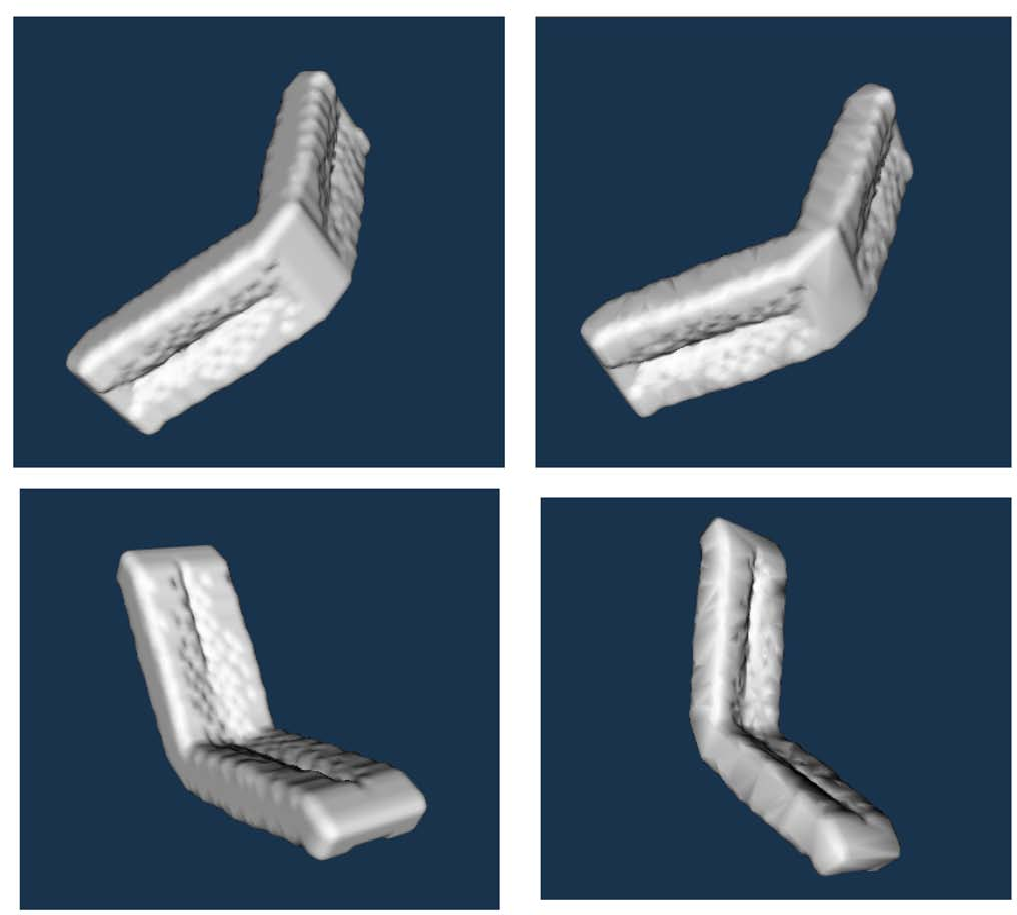
\includegraphics{Pictures/Decimation.pdf}}\\
   \caption{Decimation of triangles. \textit{Top:} 50\% \textit{Lower:} 90\%}
   \label{fig:Decimation}
\end{figure}


\section{From Parametrized Surface Points to NURBS Representation}
As of yet, there is no open-source software which provides the conversion from a \textit{mesh-based} geometry to NURBS representation. Hence, one of the main challenges of both the algorithmic and implementation part of this project has been to develop one from scratch. Due to a variety of possible approaches to tackle this problem (e.g. \cite{ eck1996automatic, becker2011advanced}), we therefore conducted extensive prototyping work in MATLAB \cite{MATLAB} to avoid cumbersome and time-consuming implementation overheads during the prototyping phase. Once the algorithms to be used had been finalized, the prototypes were implemented a non-proprietary language, Python.

Following the example of using Peters' scheme to fit NURBS smoothly to datapoints in \cite{eck1996automatic}, we did extensive prototyping to ensure the tractability of using Peters' scheme (see \autoref{subsec:peters}) for fitting a NURBS surface (see \autoref{subsub:petersleastsq}) in our settings. As mentioned above, these prototypes were done in MATLAB, and were also partly implemented in Python. 

Incorporated in these algorithms were also the least-squares fitting with a Fairness Functional term (see \autoref{subsec:fairnessthry} and \autoref{subsec:lsqfairness}) to ensure surfaces without unnecessary sharp wiggles.

In the following part of this section, the implemented algorithm will be shortly described, based on the theory and notations in \autoref{sec:NURBS} and \autoref{sec:LSQfitting}.

\subsection{Algorithm}
The algorithm is given information about a quadrilateral mesh of vertices ($\petersControlMeshVec \in \petersControlMesh$), how they are connected into quads ($\verticesof{\hat{f}}, \forall \hat{f} \in \petersFaces$) as an ordered list of four vertex indices, and how they are parameterized (parameters $(u_\lsDataPoint, v_\lsDataPoint)$ and on which quad $\hat{f}\in\petersFaces$).   roughly proceeds as follows:
\begin{itemize}
\item The information obtained from the Dual Contouring scheme is 
\item Implementations of the algorithm to calculate these \Bez point coefficients, as well as plotting them for debugging and visualisation
\item \Bez curve and surface evaluation via calculating the coefficients on each \Bez control point from a set of parameters
\item Algorithms to extract the necessary datapoints and parameters from the result data of the \acf{DC} algorithm in \autoref{ssec:DC}, using geometric conversions where necessary, and ignoring unusual datapoints
\item An algorithm for using the four above algorithms to assemble the total coefficient matrix in \autoref{eqn:petersminimisation} in \autoref{subsub:petersleastsq}
\item An application of MATLAB's built-in least squares minimisation tool to fit the resulting network of \Bez patches to the extracted surface.
\end{itemize}
A sample result, the fitting of a surface to a toroidal shape defined implicitly for the \acs{DC} algorithm is shown in \autoref{fig:fittingStructures}.


\begin{figure}
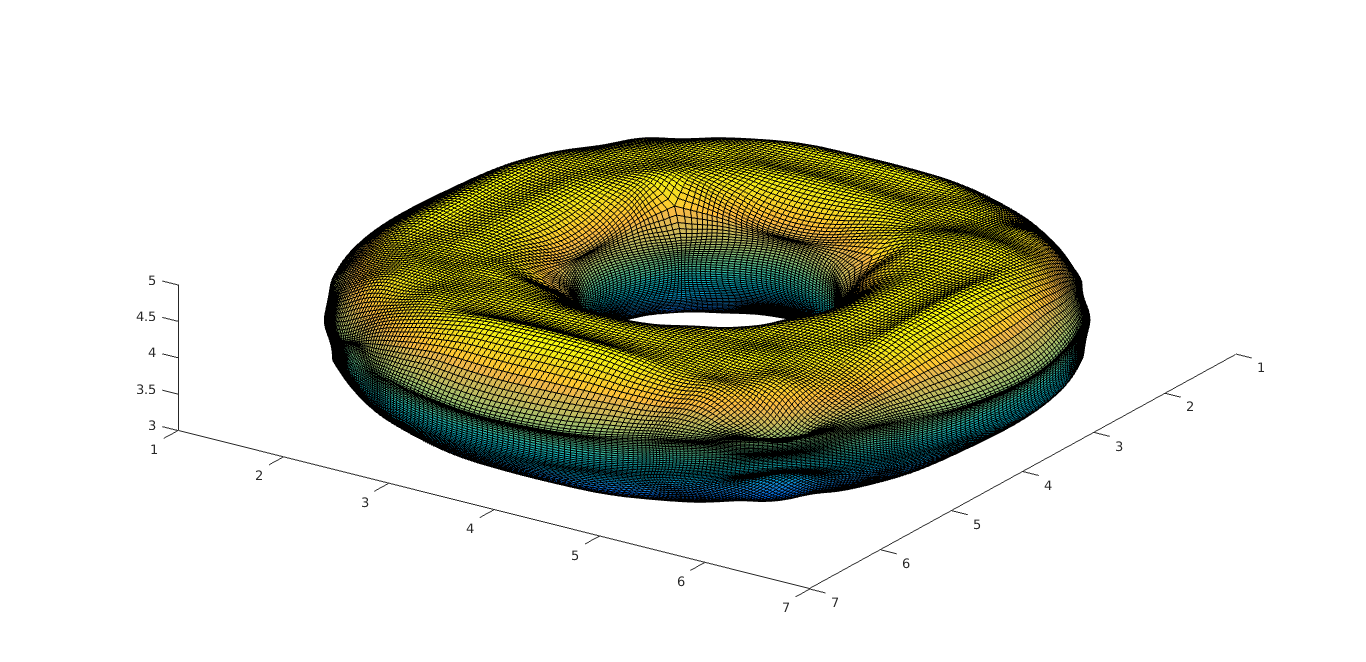
\includegraphics[width = \textwidth]{Pictures/NURBS/torus_from_DC.png}
\caption{A sample result from the Peters' scheme least-squares minimisation surface fitting, using the data provided by the \acs{DC} algorithm for an implicit function describing a torus. The grid lines on the figure are following the constant lines of each parameter value. As they follow the patch edges, corners where other than 4 coarse quads are meeting can be recognized, as for example on the middle of the far side of the torus, on the side that's facing the viewer.}
\label{fig:fittingStructures}
\end{figure}
\todourgent[inline,author=Benni]{From Bezier patches to NURBS using degree elevation. Add this to theory and implementation or only here?}



%how the algorithms were implemented



		
 ---------------------------------------------------------------------------
		%
		% Summary and discussion 
		%
 -------------------------------------------------------------------------
		\chapter{Summary \& discussion\todourgent{better caption?}}
\label{chapter:Discussion}

\section{In a nutshell:\ \acl{CADTopOpt}}
\subsection{From a \acs{CAD} model to topology optimized Voxels}
\subsection{From Voxels to Parametrized Surface Points}
\subsection{From Parametrized Surface Points to \ac{NURBS}}

\section{Future work}
\subsection{Next steps}
\todointern[inline]{what do we want to achieve until the next milestone?}
\subsection{Risks}
\todointern[inline]{what are the main risks, what might cause problems?}
\todourgent[inline]{more ugly lines... argh!!!}
		 ---------------------------------------------------------------------------
		%
		% Appendix
		%
 ---------------------------------------------------------------------------
%		\chapter{Appendix}
	%	\addcontentsline{toc}{part}{Appendix}
%		\appendix 
		
		%---------------------------------------
%		\chapter{Source Code}
%		\label{chapter:source}
%		
Here would be well-documented, nicely formatted source code.


\begin{lstlisting}[language={C++}, label={Hello World.}, frame = single ]
//include iostream for std::cout
#include<iostream>

//here beginneth the main function of the program.
int main(int argc, char * argv[])
{
	//output "Hello World" to the running terminal
	std::cout<<"Hello World!" << std::endl;
	
	//finish, returning no-error value 0.
	return 0;
}
\end{lstlisting}
		
		%\chapter{Next Appendix}
		


  	\clearemptydoublepage
  
	\bibliography{bibliography/literature}
	\todo[inline]{insert all the acronym stuff for final delivery of report}
	%\cleardoublepage
	%\printacronyms[	include-classes=abbrev,
	%				name=Abbreviations,
	%				sort = true]
	%
	%\printacronyms[	include-classes=nomencl,
	%				name=Nomenclature,
	%				sort = true]
	
 
\end{document}

